\documentclass[12pt]{cmuthesis}
\raggedbottom

%for a more compact document, add the option openany to avoid
%starting all chapters on odd numbered pages

\usepackage{comment}
\usepackage[utf8]{inputenc} % usually not needed (loaded by default)
\usepackage[T1]{fontenc}
\usepackage{url}
\usepackage{ifthen}
\usepackage{framed}
\usepackage{enumitem}
\usepackage{multirow}
\usepackage{subcaption}
\usepackage{times}
\usepackage{amssymb}
\usepackage[export]{adjustbox}
\usepackage{rotating}
\usepackage{times}
\usepackage{fullpage}
\usepackage{amsmath}
\usepackage[numbers,sort]{natbib}

\usepackage[hidelinks]{hyperref}
% \usepackage[pdfborder=0 0 0,pagebackref,pageanchor=true,plainpages=false, pdfpagelabels, bookmarks,bookmarksnumbered]{hyperref}
% pdfborder=0 0 0,  %removes outlines around hyper links in online display

\usepackage{color}
\usepackage{soul}
\usepackage{xspace}
\usepackage{makecell}
\usepackage{booktabs}
\usepackage{graphicx}
\usepackage{epsfig}
\usepackage{siunitx}
\usepackage{listings}
\usepackage{algorithm2e}
\usepackage{float}

\newenvironment{captiontext}{%
    \par\vspace{0.1in}\renewcommand{\baselinestretch}{0.9}}%
{\renewcommand{\baselinestretch}{1.0}\par}


%
% defining the \BibTeX command - from Oren Patashnik's original BibTeX documentation.
\def\BibTeX{{\rm B\kern-.05em{\sc i\kern-.025em b}\kern-.08emT\kern-.1667em\lower.7ex\hbox{E}\kern-.125emX}}


% Approximately 1" margins, more space on binding side
%\usepackage[letterpaper,twoside,vscale=.8,hscale=.75,nomarginpar]{geometry}
%for general printing (not binding)
\usepackage[letterpaper,twoside,vscale=.8,hscale=.75,nomarginpar,hmarginratio=1:1]{geometry}

% Provides a draft mark at the top of the document.
% \draftstamp{\today}{DRAFT}

\begin{document}

\frontmatter

\title{{\bf Scaling Up Wearable Cognitive Assistance for Assembly Tasks}}
\author{Roger Iyengar \\ \href{mailto:raiyenga@cs.cmu.edu}{raiyenga@cs.cmu.edu}}
\date{February 2023}
\Year{2023}
\trnumber{}

\vspace{3cm}

\committee{
  Mahadev Satyanarayanan (Satya) (Chair) \\
  Martial Hebert \\
  Roberta Klatzky \\
  Padmanabhan Pillai (Intel Labs)
}

\support{
  This work was supported by an NSF Graduate Research Fellowship under Grants
  DGE1252522 and DGE1745016.
}
% \disclaimer{}

% copyright notice generated automatically from Year and author.
% permission added if \permission{} given.

%\keywords{}

\maketitle

% \begin{dedication}

% \end{dedication}

\begin{abstract}
  Wearable Cognitive Assistance (WCA) applications run on wearable mobile
  devices, to provide guidance for real world tasks.
  Physical assembly tasks have been a significant focus of research on WCA.
  We introduce new techniques to support the development of WCA applications for
  more complex assembly tasks than previous techniques supported.
  In addition, our work reduces the load on developers creating WCA applications
  by eliminating the need to collect and label real training images.
  We accomplish this by training computer vision models on synthetically
  generated images.
  This dissertation investigates escalation to human experts in cases when a
  user is not satisfied with the automated guidance from an application.
  Lastly, we develop a new version a software framework for WCA
  applications, and evaluate ways in which WCA applications can benefit from
  running computations directly on mobile devices.
\end{abstract}

% \begin{acknowledgments}

% \end{acknowledgments}

\tableofcontents
\listoffigures
\listoftables
\mainmatter

%% Double space document for easy review:
%\renewcommand{\baselinestretch}{1.66}\normalsize

% The other requirements Catherine has:
%
%  - avoid large margins.  She wants the thesis to use fewer pages,
%    especially if it requires colour printing.
%
%  - The thesis should be formatted for double-sided printing.  This
%    means that all chapters, acknowledgements, table of contents, etc.
%    should start on odd numbered (right facing) pages.
%
%  - You need to use the department standard tech report title page.  I
%    have tried to ensure that the title page here conforms to this
%    standard.
%
%  - Use a nice serif font, such as Times Roman.  Sans serif looks bad.
%
% Other than that, just make it look good...

\chapter{Introduction}\label{chap:intro}

Wearable Cognitive Assistance (WCA) applications have been developed to help
users with tasks such as assembling physical objects, remembering people's
names, exercising, and playing games. Table~\ref{table:existing_wca} lists some
examples of WCA applications that have been developed. These applications
utilize mobile devices, such as smart glasses or a smartphone, to capture data
and interact with the user. Data is captured using sensors such as cameras.
These cameras may be mounted on glasses that the user wears, or held in a tripod
with a view of the user's workspace.
Feedback is provided in the form of synthesized speech and images shown on the
display of the mobile device.

WCA is a compelling use case for edge computing. Many of these applications
utilize large deep neural network (DNN) models that are too computationally
intensive to run on a small and lightweight mobile device. However, these
applications generate large volumes of data that must be processed quickly.
Therefore, computation must be offloaded to a server with close network
proximity to the mobile device that is capturing the data~\cite{satya14}. We
will henceforth refer to this server as a cloudlet.

This work focuses on WCA applications that help users complete physical
assembly tasks.
Users are given step by step instructions, which requires the application to
determine when a user has completed a step of the task. Applications have been
developed for a lego kit~\cite{lego}, a lamp~\cite{lamp}, and a toy
sandwich~\cite{sandwich}. These tasks all required fewer than ten steps and
used parts that had distinct shapes and colors.
Taking WCA applications to the next level will require supporting tasks with
many more parts, many more steps, parts that are small relative to the full
object being assembled, and a combinatorial explosion of error states.
We propose to address these challenges in this research.

One significant challenge is the amount of labeled data that is required for
training computer vision models. Each
step of the task, and every error state that the developer would like to detect,
must be represented in the data that the models get trained on.
Increasing the number of steps thus directly increases the amount of data that
is required for training the models.
Collecting and labeling all of this data is an incredibly time-consuming
process.
This process can take up to 2 or 3 hours per task step.
Developing these models is an iterative process, which involves testing under
different lighting conditions, and then collecting more data in environments
that the model performs poorly in.
Creating training sets is thus a significant barrier to developing WCA
applications that support large numbers of steps and large numbers of parts.

As the number of parts being assembled increases, the size of the final object
does as well. An object made out of 100 parts is going to be significantly
larger than some of the individual parts. The camera is going to capture images
of the full object, but the application needs to determine when each individual
part has been inserted into the correct location on the full assembly.

Machine Learning models for computer vision require training data for each
object that the model will detect. Detecting every possible error state using
such a model would require collecting and labeling data for each of these
possible states.

\subsection{Thesis Statement}

\textbf{
  Scaling up WCA to complex assembly tasks is challenging because of
  (a) the difficulty of
  vision-based state detection with very small parts in the context of much
  larger objects being assembled; (b) the combinatorial explosion
  of possible error states; and (c) the large manual effort needed to create
  accurate DNNs that can reliably determine when task steps have been completed.
  These problems can be solved by a combination of (1) hierarchical
  decomposition of
  complex assemblies into modular compositions of subassemblies, (2) on-demand
  seamless
  escalation for live expert assistance, and (3) synthetic generation of
  training
  sets for born-digital components. The resulting solution can be implemented in
  a scalable and maintainable way using modular software components.
  This will enable the development of WCA applications for more complex tasks,
  which is a necessary step along the path towards making WCA applications
  practical for real world tasks.
}

\chapter{Background}\label{chap:background}

\section{Aids for Assembly Tasks}

We have found a large body of work on systems to aid with assembly tasks.
However, none of these systems determined when steps were completed using
computer vision models that processed data from an RGB camera. The techniques we
propose do not require instrumenting parts of workspaces with sensors. Our
system also does not require the person who is completing the task to determine
when a step has been completed, and then indicate this to the system. On top of
this, our system only starts a call with a task expert when the person
completing the task has reached an error that the computer vision models cannot
handle.
This burdens task experts much less than a system where the task expert must be
on a call to help a user with the full task.

\citet{webuild} developed a system to distribute steps for an assembly task
among members of a group completing the task together. Instructions are
displayed on a smartphone screen, and users manually press a
button to indicate when a step is completed.
The authors ran a user study where people assembled an IKEA cabinet and a
Meccano bridge kit.
Requiring people completing the task to indicate when a step is completed
creates an additional burden that our system avoids.
\citet{sensors} developed a system that
determines when steps for assembling an Ikea wardrobe have been completed, using
sensors such as gyroscopes, accelerometers, force sensing resistors, and
infrared distance meters. This system allows users to complete steps of the task
in different orders.
However, their system was purely focused on detecting completed steps, and it
did not give the users any instructions.
\citet{kinect} used a Kinect
sensor to guide users through assembling objects out of Duplo blocks. The system
determined when steps were completed by processing data from the Kinect sensor.
Duplo blocks have bright colors and simpler shapes than the objects that our
tasks use.
\citet{smartwatch} developed a system that provides instructions to users on
smartwatch displays, and determines when steps have been completed using sensors
that are typically present in a factory environment, such as RFIDs and infrared
light barriers~\cite{smartwatch2}.
Our system does not require the presence of such sensors.

\citet{robotic_arm}'s system guided users through assembling a pavilion out of
bamboo sticks. The users moved around a room, picking up certain sticks and
then delivering them to a robotic arm. Users wore Apple Watches, and were given
written instructions on the watches' displays. A user swiped on the face to see
the next instruction. The locations of each user were also tracked using BLE
beacons that communicated with iPhones that users carried. A centralized system
used the location information to decide the next instruction that should be
given to each user.
This system requires users to manually request the next instruction, while our
system automatically gives the next instruction after the user completes a step.

\citet{collaboration} examined systems where remote experts helped users with
assembly tasks. The people completing tasks communicated using a tablet for one
task, and a Google Glass for another. In addition,
they looked at a case where where the user could stay in one place and a case
where the user had to move across different workspaces to complete the task.

Table~\ref{table:prior_work} provides a brief summary of all of the existing
systems described in this section.

\begin{table*}
  \begin{tabular}{| l | p{2in} | p{2.5in} |}
    \hline
    Prior Work & Detection of Step Completion & Other Attributes\\
    \hline
    \citet{webuild} & User presses a button & Multiple users working on task
                                              together.\\
    \hline
    \citet{sensors} & Automatic, using gyroscopes, accelerometers, force sensing
                      resistors, and more & Requires sensors to be installed in
                                            the Ikea parts. Did not give
                                            instructions.\\
    \hline
    \citet{kinect} & Automatic, using Microsoft Kinect & Builds a full virtual
                                                         model of what the user
                                                         has constructed. Only
                                                         supports large colorful
                                                         duplo blocks. \\
    \hline
    \citet{smartwatch} & Automatic, using RFIDs and infrared light barriers
                                              & Requires sensors to be present
                                                in working environment.\\
    \hline
    \citet{robotic_arm} & Manually from user
                                              & The final assembled object was
                                                massive. Many parts were
                                                identical.\\
    \hline
    \citet{collaboration} & Remote task expert
                                              & Compared Tablet with Google
                                                Glass.\\
    \hline
\end{tabular}
\caption{
  Existing systems that helped users with physical assembly tasks.
}\label{table:prior_work}
\end{table*}

\section{Wearable Cognitive Assistance}

\begin{table*}[h!]
\centering
\begin{tabular}{|p{0.40in}|p{1in}|p{3.2in}|p{0.7in}|p{0.8in}|}
\hline
App Name & Example Input Video Frame & Description & Symbolic Representation & Example Guidance \\
\hline
\textbf{Pool} & \raisebox{-0.9\totalheight}{\includegraphics[width=0.97in]{figures/table_existing/example-pool.png}}
&
Helps a novice pool player aim correctly. Gives continuous visual feedback (left arrow, right arrow, or thumbs up) as the user turns his cue stick.  The symbolic representation describes the positions of the balls, target pocket, and the top and bottom of cue stick.
&
$<$Pocket, object ball, cue ball, cue top, cue bottom$>$ &  \raisebox{-0.85\totalheight}{\includegraphics[width=0.8in]{figures/table_existing/guidance-pool.png}} \\
\hline
 \textbf{Ping-pong} & \raisebox{-0.9\totalheight}{\includegraphics[width=0.97in]{figures/table_existing/example-pingpong.png}}
&
Tells novice to hit ball to the left or right, depending on which is more likely to beat opponent. Uses color, line and optical-flow based motion detection to detect ball, table, and opponent.  Video URL: {\em https://youtu.be/\_lp32sowyUA}
&
 $<$InRally, ball position, opponent position$>$ & ``Left!'' \\
\hline
 \textbf{Work-out} & \raisebox{-0.9\totalheight}{\includegraphics[width=0.97in]{figures/table_existing/example-workout.png}}
&
Counts out repetitions in physical exercises. Classification is done
using Volumetric Template Matching on a 10-15 frame video segment.  A
poorly-performed repetition is classified as a distinct type of
exercise (e.g. ``good pushup'' versus ``bad pushup'').
&
 $<$Action, count$>$ & ``8'' \\
\hline
 \textbf{Face}     & \raisebox{-0.9\totalheight}{\includegraphics[width=0.8in]{figures/table_existing/example-face.png}}
&
Jogs your memory on a familiar face whose name you cannot recall. Detects and extracts a tightly-cropped image of each face, and then applies a state-of-art face recognizer. Whispers the name of the person recognized.
&
 ASCII text of name & ``Barack Obama'' \\
\hline
 \textbf{Lego} & \raisebox{-0.9\totalheight}{\includegraphics[width=0.9in]{figures/table_existing/example-lego.png}}
&
Guides a user in assembling 2D Lego models.  The symbolic representation is a matrix representing color for each brick.   Video URL: {\em https://youtu.be/7L9U-n29abg}
&
 [[0, 2, 1, 1], \break [0, 2, 1, 6], \break [2, 2, 2, 2]] \break & ``Put a 1x3 green piece on top'' \\
\hline
 \textbf{Draw} & \raisebox{-0.9\totalheight}{\includegraphics[width=0.9in]{figures/table_existing/example-draw.png}}
&
Helps a user to sketch better. Builds on third-party app for desktops. Our implementation preserves the back-end logic. A Glass-based front-end allows a user to use any drawing surface and instrument. Displays the error alignment in sketch on Glass.  Video URL: {\em https://youtu.be/nuQpPtVJC6o}
&
\raisebox{-0.85\totalheight}{\includegraphics[width=0.7in]{figures/table_existing/symbolic-draw.png}} & \raisebox{-0.95\totalheight}{\includegraphics[width=0.7in]{figures/table_existing/guidance-draw.png}} \\
\hline
 \textbf{Sand-wich} & \raisebox{-0.9\totalheight}{\includegraphics[width=0.97in]{figures/table_existing/example-sandwich.png}}
&
Helps a cooking novice prepare sandwiches according to a recipe. Since real food is perishable, we use a food toy with plastic ingredients. Object detection uses Faster-RCNN deep neural net approach.~\cite{frcnn}

    Video URL: {\em https://youtu.be/USakPP45WvM}
&
 Object: \break ``E.g. Lettuce on top of ham and bread'' & ``Put a piece of bread on the lettuce'' \\
\hline

\end{tabular}
\caption{Example Wearable Cognitive Assistance Applications. The input frame is
  sent to a cloudlet, which converts it to the symbolic representation. The
  symbolic representation is then used to give guidance.
  (Source: Adapted from Satyanarayanan~\cite{Satya2017})
}\label{table:existing_wca}
\end{table*}

A WCA application provides just-in-time guidance and error detection for a user
who is performing an unfamiliar task.
Prompt error detection is also valuable for a user who is performing familiar
tasks, since human errors cannot be completely avoided, especially when the user
is tired or stressed.
Informally, WCA is like having ``an angel on your shoulder.''~\cite{ha2014}
It broadens, the metaphor of GPS navigation tools that
provide real-time step-by-step guidance, with prompt error detection and
correction.

Table~\ref{table:existing_wca} lists some examples of WCA applications that we
have developed.
In total, we have developed over 15 WCA applications.
This thesis focuses on applications that that help users assemble physical
objects.
We have developed such applications for an IKEA lamp, a Lego kit, a toy
sandwich, an IKEA cart, and a Stirling engine.

These applications are a compelling use case for edge computing.
They first capture images using the camera on a mobile device, such as a
smartphone or head-mounted wearable device.
The images are then sent to a cloudlet for processing, using the Gabriel
platform~\cite{ha2014}.
The computational limitations of lightweight mobile devices that have acceptable
battery life prevent us from being able to process these images using the
devices' own hardware~\cite{Satya2009}.
Table~\ref{fig:wca_apps} lists the resource consumption and end-to-end latency
bounds of five offloading-based WCA applications.
It shows that WCA applications are simultaneously compute-intensive,
bandwidth-hungry, and latency-sensitive.

\begin{table*}
  \centering
    \begin{tabular}{|l||c|c|c|c|c|}
    \hline
    & Pool & Ping-pong & Face & Lego & Sandwich \\
    \hline
    \hline
    Cloudlet CPU load(\%) & 72.10 & 45.40 & 75.60 & 52.20 & 85.10 \\
    \hline
    End-to-end latency bounds (tight--loose, ms)* & 95--105 & 150--230 & 370--1000 & \multicolumn{2}{c|}{600--2700} \\
    \hline
    Video streaming bandwidth requirement    & \multicolumn{5}{c|}{480p:~~ 3.6 / 7.0} \\
    ~~~~~(Average / Peak, Mbps)              & \multicolumn{5}{c|}{720p:~~ 6.8 / 9.9} \\
                                             & \multicolumn{5}{c|}{1080p:~~ 8.1 / 12.7} \\
    \hline
    \end{tabular}
    \caption{CPU load, latency bounds, and the required bandwidth of example WCA applications.
	The implementations of the application servers~\cite{chen2017} were tested on a laptop (with an Intel$^{\mbox{\footnotesize\textregistered}}$ Core$^{\mbox{\footnotesize\texttrademark}}$ i7-8500Y processor and 8GB RAM), running the frontend on an Android phone, using 480p, 720p, and 1080p video resolutions.
    (*) End-to-end latency includes both the round trip time (RTT) from the Android phone to the cloudlet and compute time in the cloudlet.
	Tight and loose bounds are adopted from Chen, et al,~\cite{chen2017} where they are defined:  ``The tight bound represents an ideal target, below which the user is insensitive to improvements. Above the loose bound, the user becomes aware of slowness, and user experience and performance is significantly impacted.''
    }\label{fig:wca_apps}
\end{table*}

\subsection{WCA Tools}

\citet{ha2014}
introduced the first version of a programming framework called Gabriel. This
framework includes networking and runtime components for WCA applications.
\citet{chen2017} developed an initial set of WCA applications, determined
how much latency was acceptable for these applications, and examined how changes
to the network, hardware, and algorithms used can affect end to end latency.
\citet{wang2019} examined how to reduce  the load imposed
on a cloudlet by a single WCA user, thereby allowing many more
users to share single cloudlet.
\citet{pham2021ajalon} developed a toolchain that
allows people to develop WCA applications without writing any code.

\section{Computer Vision}

\citet{gebru2017finegrained} used a two step process to find and distinguish
cars
that appeared in Google Street view images. Their first step was finding the
regions of images that were likely to contain cars. Then their second step was
classifying the type of car in that region. We will train models on our own new
data, but these models will use existing neural architectures.

Image classifiers give a single class label for a full image, and do not provide
a bounding box. These are most useful when a scene has already been cropped to a
region involving a single object. Imagenet~\cite{ImageNet_VSS09} is a
classification dataset which contains classes for 1000 objects. Object
detectors provide bounding boxes and labels for objects in an image. This is
particularly helpful
when an object might only take up part of the camera view, or there might be
multiple objects visible
at once. Microsoft COCO~\cite{coco} is an object detection dataset with 80
classes.

Faster R-CNN~\cite{frcnn} is an object detector that is used in our
lamp~\cite{lamp} and toy sandwich~\cite{sandwich} assembly assistants.

Imagenet has the classes ``race car,'' ``sports car,'' and ``streetcar,''
in addition to classes for objects that aren't cars. The Stanford Cars
dataset~\cite{KrauseStarkDengFei-Fei_3DRR2013} is more fine-grained, with
images of cars that are labeled with the year, make, and model.
The Fast MPN-COV~\cite{Li_2018_CVPR} image classifier performs
well on several fine-grained classification datasets.

Object detectors have been used for finding screws in pictures of aircraft
parts~\cite{visapp19} and consumer electronics~\cite{FOO2021666}.
\citet{wu2018spot} found differences between book covers using a modified
version of Faster R-CNN.

\subsection{Synthetic Training Data}

The idea of avoiding manual labeling has a long and rich history.
\citet{synthetic} trained an object detector on synthetic data that
outperformed an object detector trained on real data. They generated backgrounds
cluttered with distractor objects. In addition, they added some distractor
objects to the foreground and varied the lighting conditions that were used to
render each of the images. These images looked 3D, but they were not
photo-realistic. Other works have generated photo-realistic images to use as
training data~\cite{DBLP:journals/corr/abs-1809-10790, photo2}, or used real
background images~\cite{real_background1, real_background2, real_background3}.
\citet{dwibedi} avoided rendering 3D graphics altogether by cropping objects
from photographs, and pasting these crops into other photographs.
Their models trained on synthetic images performed worse than their models
trained on real images.
However, they also  trained models using a mix of real and synthetic images, and
these performed better than models trained on real or synthetic data alone.

\section{Hierarchical Decomposition}

\citet{Simon1991} argued that all complex systems are made up of smaller
systems. These smaller systems are made up of even smaller systems, thus
forming a hierarchy with several layers.
Reasoning about a smaller system on its own is easier than trying to understand
a full system all at once.
We can apply this idea to state detection for WCA applications by decomposing
a large assembly task into separate sub-assemblies with 8-10 parts.
This limits the scope of what any one computer vision model that we use is
responsible for.
It also allows multiple developers to work on computer vision models for
different parts of the task completely independently from each other.
Finally, it also simplifies performance of a task over an extended period
(e.g. multiple days). A person who has to stop work in the middle of a task will
have an easier time if the task is split into subtasks that don't require any
context from earlier subtasks. They can start work from the beginning of a
subtask every time, rather than having to recall anything about steps they
completed the last they they worked on the task.

\citet{semantic_hierarchy} utilized hierarchies of visual features to recognize
objects.
\citet{subassembly_identification} automatically identified subassemblies of
assembled objects based on CAD files.
They utilize features such as the number of other parts that a certain part
touches, or the amount of surface area that two touching parts share.
They considered subassemblies from the perspective of assembly sequence
planning, rather than detecting completed task steps using computer vision.

\chapter{Detecting Completed Steps}\label{chap:detection}

A WCA applications for a physical assembly task must detect when a step of the
task has been completed.
A user wears a mobile device with a camera (such as a Google Glass).
The mobile
device gives the user an instruction, waits for them to complete this, and then
gives them the next instruction.
Completing a step might require adding a part to the assembly,
removing a part from the assembly, or repositioning the object in order to give
the camera a certain view.
The application must determine when a step is completed
based on images from the camera.
It is important to avoid false positives, which are instances where the
application determines that a step has been completed before it actually has
been.
False positives cause the application to give the user a new instruction before
the previous step gets completed, which results in a poor user experience.

\section{Hierarchical Decomposition}

An object made up of many parts is going to be larger than most of the
individual parts.
Rather than asking the user to move their head close to each part
they install, the system should be able to determine when a step has been
completed based on an image that contains most or all of the full object being
assembled.
Breaking up a large object into a collection of sub-assemblies makes
this possible.
Our system uses a two stage process where it first finds the
region of an image that contains the sub-assembly involved in a step. It then
crops the image around this region, and the next model determines if the step
has been completed based on the cropped image. Inspired by Simon's argument that
all complex systems are made up of smaller systems~\cite{Simon1991}, we argue
that any object that is assembled from more than ten parts can be decomposed
into sub-assemblies.
Hence the hierarchical approach proposed here can be scaled upwards, without
obvious limits.

This technique is applicable to tasks
with multiple levels of sub-assembly hierarchies.
An assistant for a task involving multiple sub-assemblies is effectively a
series of independent applications. Once the user completes one sub-assembly,
they will automatically be taken to the assistant for the next one.
If the
sub-assemblies must be connected together after that, there will be an assistant
for these steps as well.
Tasks can be broken into sub-assemblies the same way that long documents can be
broken into chapters, sections, and subsections.
Sub-assemblies near the top of the hierarchy are going to be made up of multiple
levels of sub-assemblies below them.

Figure~\ref{fig:stirling_full} shows two of the sub-assemblies of a Stirling
engine.
Our application uses a different pair of computer vision models for each
sub-assembly.
The code selects the correct pair based on the current step that the user is
working on.
Each step involves removing a piece from one sub-assembly.
None of the sub-assemblies involve more than 8 steps.
Splitting the task up into sub-assemblies thus simplifies the scope of the
problem to developing a set of assistants for 8 step tasks.

The number of steps required for each sub-assembly is not something that we have
any fixed rules about. We have found that limiting the number of steps to 10
appears to work well empirically, but the optimal number of steps for a
sub-assembly will likely vary based on the task.

\begin{figure}

  \includegraphics[width=7cm]{figures/stirling/full.png}
  \caption{A stirling engine with two sub-assemblies highlighted
  }\label{fig:stirling_full}
\end{figure}

Figure~\ref{fig:erector} shows how a model motorcycle can be broken up into
three sub-assemblies.
The Stirling engine has a single large base, but the motorcycle is simply
assembled from small pieces. Therefore, assembling the motorcycle would require
an additional set of steps at the end, to connect the sub-assemblies together.

\begin{figure}
  \begin{subfigure}{\textwidth}
    \includegraphics[width=5cm]{figures/erector/full.jpg}
    \caption{The fully-assembled model}
  \end{subfigure}
  \begin{subfigure}{\textwidth}
    \includegraphics[width=5cm]{figures/erector/sub1.jpg}
    \includegraphics[width=5cm]{figures/erector/sub2.jpg}
    \includegraphics[width=5cm]{figures/erector/sub3.jpg}
    \caption{Sub-assemblies}
  \end{subfigure}
  \caption{A model motorcycle from a Meccano Erector kit
  }\label{fig:erector}
\end{figure}

\subsection{Implementation}

Our applications accomplish hierarchical decomposition by processing camera
images using a two stage process inspired by \citet{gebru2017finegrained}.
The first stage involves finding the region of the
image that contains the subassembly that a user is working on, using Faster
R-CNN~\cite{frcnn}.
Next, the image is cropped around this region, and the cropped region is
classified using Fast MPN-COV~\cite{Li_2018_CVPR}.
There is one Fast MPN-COV per subassembly.
The Fast MPN-COV model has one label for each step of the task that is part of
this model's subassembly.
The classification result therefore indicates the step of the task that is shown
in an image.
The application considers a step to be complete when an image from the camera
feed is classified as the label corresponding to the next step.
The architecture for this application is shown in Figure~\ref{fig:arch}.

\begin{figure}
  \includegraphics[width=\columnwidth]{figures/architecture.pdf}
  \caption{
    The architecture of our WCA application for the Meccano erector kit.
    The dashed lines represent a Wi-Fi connection.
    The solid lines represent a connection over Gigabit Lan.
    The dotted lines represent data transmission between components on a single
    cloudlet.
  }\label{fig:arch}
\end{figure}

A single label may correspond to multiple steps of a task.
For example, a kit might contain two identical subassemblies that get assembled
on their own, before being connected to the rest of the kit.
The steps required to assemble both of these subassemblies will be identical.
The subassemblies do not get connected to the rest of the kit until after they
have been assembled, so there will not be any visible differences while the user
is assembling one or the other.
The application can therefore use the same sequence of outputs from a computer
vision model for both subassemblies.
However, two consecutive steps cannot share the same label.
The application considers a step to be completed when images are classified with
the label corresponding to the next step.
If the next step had the same label, the application would think that the user
completed a step immediately after the step was started.
This issue is illustrated in Figure~\ref{fig:consec_step}.

\begin{figure}
  \includegraphics[width=\columnwidth]{figures/consec_step.pdf}
  \caption{
    The sequence of steps depicted in the top row cannot be supported by our
    techniques because the two consecutive steps are identical.
    The sequence of steps depicted in the bottom row is acceptable because the
    identical steps are not consecutive.
  }\label{fig:consec_step}
\end{figure}

\subsubsection{Training}

We performed transfer learning from pre-trained models, rather than training
models from scratch.
Our Fast MPN-COV models were pre-trained on ImageNet 2012~\cite{ILSVRC15} and
our Faster R-CNN models were pre-trained on COCO 2017~\cite{coco}.
We used a PyTorch~\cite{pytorch} implementation of Fast MPN-COV and a
TensorFlow~\cite{tensorflow2015-whitepaper} implementation of Faster R-CNN.

\subsubsection{Error Correction}

Developers can train fine-grained classifiers to recognize specific mistakes
that a user of a WCA application might make when trying to complete a task.
An error state requires training data, the same way other steps of the task do.
When a frame gets classified as depicting an error state, the user is given
instructions about how to correct this.
Chapter~\ref{chap:escalation} provides further discussion about handling errors
with WCA applications.

\subsubsection{Development Tools}

We expanded the Ajalon tools~\cite{pham2021ajalon} to support hierarchical
decomposition.
Ajalon previously only supported a single object detector, which was sufficient
for toy examples such as the sandwich described in~\cite{chen2017}.
However, more complex assembly task require the use of multiple object detectors
and multiple fine-grained image classifiers.
Our improvements to Ajalon allow developers to have the application use
different computer vision models as a user progresses through a task.
This results in a single application that will automatically start
giving users instructions for the next sub-assembly after they have completed
the previous one.

\section{Our Applications}

To validate our approach, We developed WCA applications for three real assembly
tasks.
We trained models for these applications using real videos that were recorded
using a smartphone.
The videos were manually annotated with bounding boxes using CVAT.
We cleaned up our dataset by computing the perceptual hash values of every
image.
For all sets of images with identical perceptual hash values, we removed all but
one of the images.
This resulted in a set of images that all had unique perceptual hash values.

We have posted\footnote{\url{https://rogeriyengar.com/thesis}} all of the
artifacts required to run these applications, along with videos showing them
being used.

\subsection{Stirling Engine}\label{sec:stirling}

This WCA application guides users through disassembling a
Stirling engine.
This task requires 22 steps. All of the parts are made out of
metal, with the exception of one ring that is made out of silicone. Some steps
just require removing a single screw, and the engine looks very similar before
and after these steps have been completed.
We split the task into four subassemblies, which are shown in
Figure~\ref{fig:stirling_subs}.

\begin{figure}
  \includegraphics[width=\columnwidth]{figures/stirling_subassemblies.pdf}
  \caption{
    The steps detected by our Stirling Engine WCA application.
    The blue rectangles represent subassemblies.
    Each subassembly corresponds to a different Fast MPN-COV model.
  }\label{fig:stirling_subs}
\end{figure}

Several steps of the task involved removing screws from the engine.
The labels for these steps indicated the number of screws visible in the frame,
rather than being unique to the specific step of the task.
For example, in Figure~\ref{fig:stirling_steps}, the first and third steps
were both given the label ``2 Black Screws.''
The training script for Fast MPN-COV randomly flips images
horizontally, so we did not want the label to depend on the orientation of
objects.
The initial steps for this task all require removing screws or flipping the
engine to show screws that were previously occluded.
Therefore, every step changes the number of screws that are visible.

\begin{figure}
  \includegraphics[width=\columnwidth]{figures/stirling_steps.pdf}
  \caption{Four states from our WCA application for a Stirling engine. The
    steps look visually similar aside from the number of screws that are
    visible. The text in colored boxes are the labels that our image classifier
    was trained on.
    Note that some different steps were given the same label, but consecutive
    steps must have different labels.
    The text in the white boxes describes the actions users take to complete a
    step.
  }\label{fig:stirling_steps}
\end{figure}

We found that illuminating the engine with a table lamp increased the accuracy
of the application beyond what we could achieve with overhead room lighting.
We lit the object the same way when capturing training data and using the
application.

\subsection{Ikea Cart}\label{sec:ikea_cart}

Our next application provides guidance for users assembling an Ikea Raskog
utility cart.
The task requires twenty steps to complete successfully.
However, the cart has two pairs of identical components that must be
assembled the same way.
Therefore, four of the steps are repeats of earlier steps.
The application uses the same label in cases where steps are identical.
Thus there were 16 labels, that each corresponded to the 16 unique steps.
In addition, we developed the application to detect one error state, so there
were 17 possible labels that our models could output.
We split the task into three subassemblies, which are shown in
Figure~\ref{fig:ikea_cart}.

The repeated steps are repeated in pairs. For example, step 1 is performed,
followed by step 2.
Then both are repeated.
Repeating steps in pairs avoids the situation where two consecutive steps
correspond to the same label from the classifier.

\begin{figure}
  \includegraphics[width=\columnwidth]{figures/ikea_subassemblies.pdf}
  \caption{
    The steps detected by our Ikea WCA application.
    The blue rectangles with rounded corners represent subassemblies.
    The steps in the rectangles without rounded corners are repeated.
    The error state appears in the red circle.
  }\label{fig:ikea_cart}
\end{figure}

\subsection{Toy Car}

The last application guides users through assembling a model car.
This task requires 28 steps, which we split into 6 subassemblies.
These steps and subassemblies are shown in Figure~\ref{fig:toy_car}.
The computer vision models output a unique label for each step of the task.

\begin{figure}
  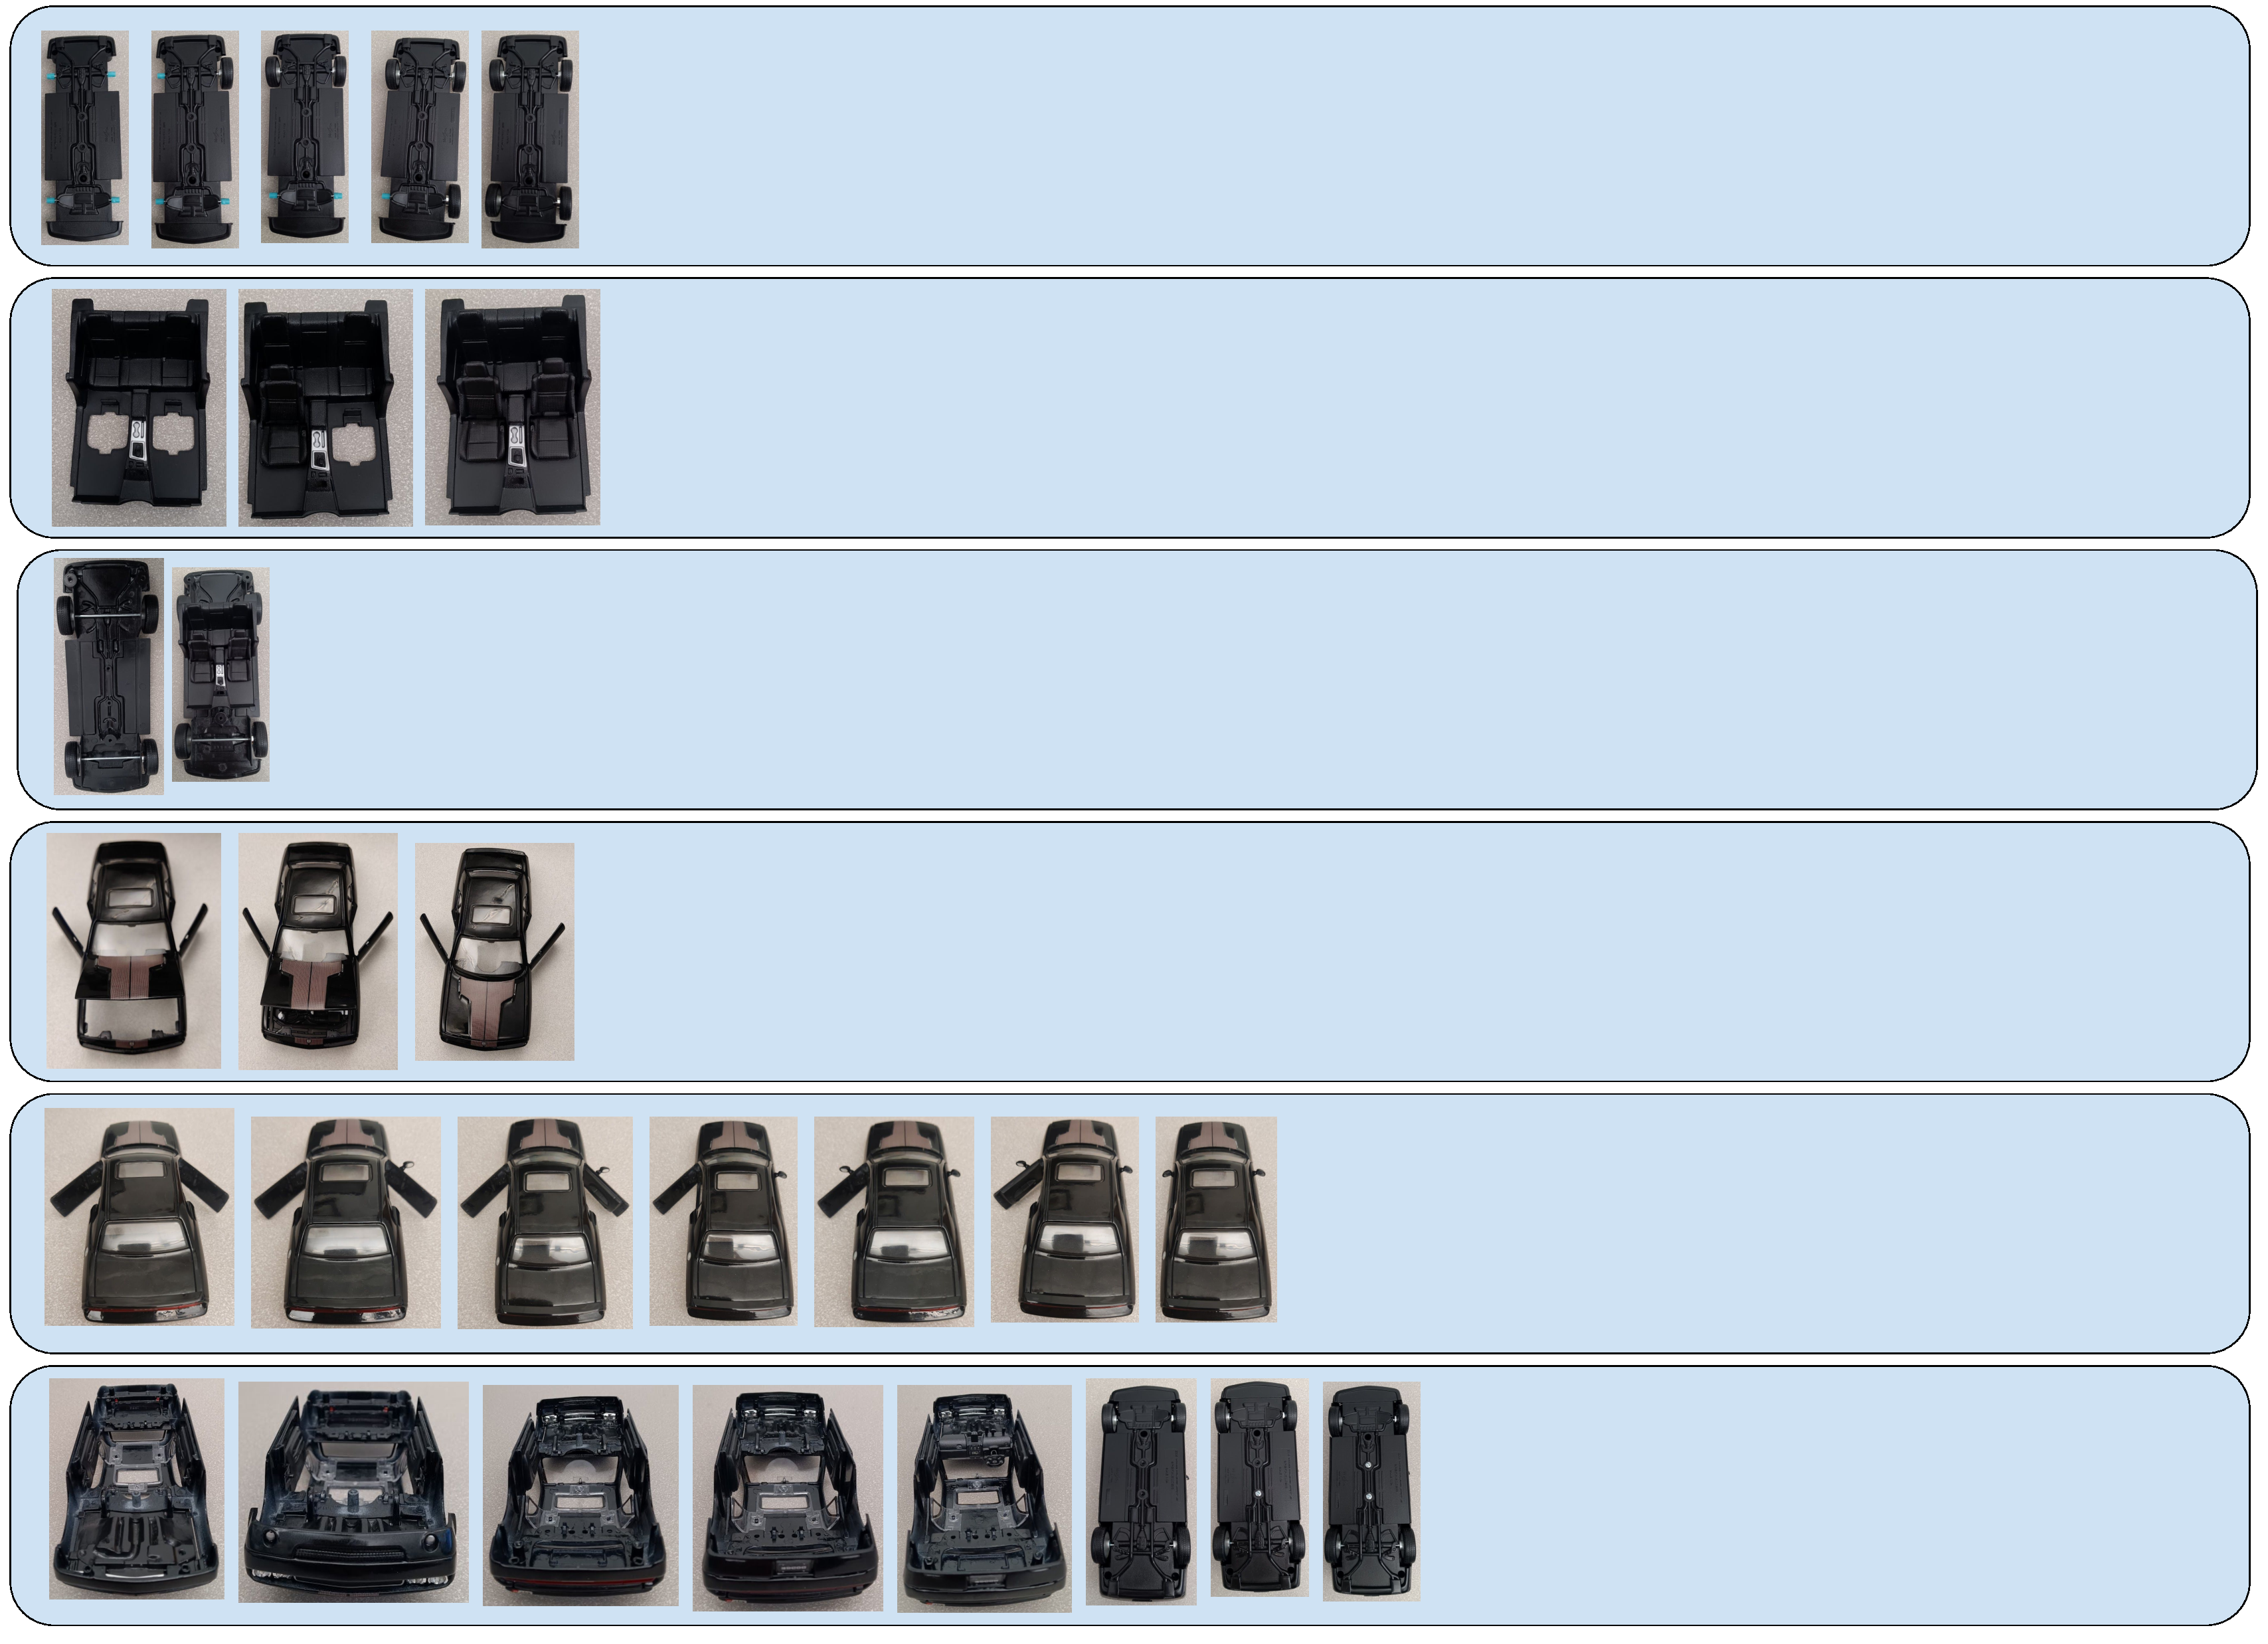
\includegraphics[width=\columnwidth]{figures/toycar_subassemblies.pdf}
  \caption{
    The steps detected by our Toy Car WCA application.
    The blue rectangles represent subassemblies.
  }\label{fig:toy_car}
\end{figure}

\section{Implementation Details}

We captured images at 1920x1080 pixels, and transmitted these to the cloudlet at
their full resolution.
This is the highest resolution that Android CameraX's ImageAnalysis use case
supports.
After processing the images with Faster R-CNN, the application crops them around
the region that likely contains the object.
The cropped image is resized to 448x448 pixels and then classified by Fast
MPN-COV.
By starting with a large initial image, we ensured that the cropped image would
be at least 448x448 pixels.

\subsection{Realtime Data}

The code for many computer vision models are written to run inference on batches
of images that are stored on disk. The torchvision package contains functions
for loading images from disk, in batches. Using these models in WCA applications
requires modifying the code to run the models on images being transmitted over
the network, one by one. The input batch size must be set to 1, because anything
larger would require building up a queue of images that would be run through the
model together as a single input. A larger batch size would improve the
frame rate for inference, but hurt the latency.

Live data must be as similar as possible to the data that the models are trained
on. For example, converting a
JPEG image to raw pixel values using OpenCV will result in slightly different
values than using Pillow will. We observed that our Fast MPN-COV model performed
significantly better with images opened using Pillow than with images opened
using OpenCV. The training images were opened using Pillow, but we did not
expect opening JPEGs with OpenCV and Pillow to result in different color values.

Processing images while a user is in the middle of a step wastes bandwidth and
computing resources on cloudlets.
In addition, it might lead to an application mistakenly
believing that a step has been completed before it actually has been.
We experimented with a filter that requires a set of consecutive frames to have
identical perceptual hash values.
This essentially means that a certain number of images in a row all had to look
the same.
This technique worked well for WCA applications running on a smartphone mounted
to a tripod.
But it did not work well for WCA applications running on a Google Glass, due to
the motion of the user's head.
Instead, we required a sequence of sequential images to be assigned the same
label by the classifier.
This helped avoid cases where the application mistakenly believed a step had
been completed while a user was still in the middle of it.
But it did not save computing resources on the cloudlet, because every frame had
to be processed.

\chapter{Synthetic Training Images}\label{chap:synthetic}

Training the DNNs that are used by WCA applications for physical assembly tasks
requires thousands of labeled images.
Capturing and labeling these images requires substantial effort.
Bounding boxes must be drawn around the region of each image that
contains the object being assembled.  The bounding box must then be
labeled with the step of the assembly process that is depicted in the
image.  Collecting and labeling a training set of images is a major
barrier to entry for anyone who wants to develop a WCA application for
a new task.
For example, this effort took over 50 person hours for the Ikea Cart application
described in Section~\ref{sec:ikea_cart}.
This task had 17 different states.
This time-consuming and labor-intensive
aspect of WCA is the biggest bottleneck to its widespread adoption.

Previous papers have proposed the use of synthetically generated
images for training sets.  In this approach, pre-labeling is done by
construction~\cite{synthetic_data, DBLP:journals/corr/abs-1809-10790,
  photo2, real_background1, real_background2, real_background3,
  dwibedi}.  Since programs that generate synthetic images have
information about the objects that are visible and their locations,
there is no need for manual input of this information.  In addition,
synthetic images of objects can easily be rendered in a wide variety
of different lighting conditions and environments.  In contrast,
capturing real images of objects in a variety of conditions requires
the images of the object to be captured in every such environment.
Overall, the use of synthetic data may save considerable manual
effort.

This chapter presents our experience training DNNs for WCA applications for
three assembly tasks, using synthetic training images.

\section{Meccano Erector Kit}

In this section, we ask how well synthetic images work for creating a WCA
application for assembling a Meccano Erector Kit.
We use the following procedure to answer this
question.  We first generate a set of synthetic (pre-labeled) images
using the Unity Perception package~\cite{unity}.
Unity is a video game engine that includes 3D graphics rendering capabilities
and CAD tools.
The Perception package was created by Unity to enable the creation of object
detectors from CAD models instead of real images, that had to be labeled with
bounding boxes.

After generating the synthetic images with Unity, we train
computer vision models on this data.  Next, we  collect and manually
label a set of real images for the same task, and then train computer
vision models on this data.  Finally, we compare the accuracy of these
two families of models on a held-out test set of real images.  Our
results show that models created with a training set size of 75,000
synthetic images perform slightly better than models created with
roughly 15,000 real images.
However, this ordering is reversed when fewer synthetic images are used for
training.

The Meccano Kit assembles into a model bike.
The fully assembled model is depicted in Figure~\ref{fig:full_bike}.
It is made from over 50 parts.
However, this work will only separate the bike into three subassemblies.
The fine-grained classifiers we trained for this kit had 5 output labels.
Three of the labels were for the individual subassemblies, and the remaining two
were for the steps required to put the subassemblies together.

\begin{figure}
  \includegraphics[width=\columnwidth]{figures/synthetic/full_bike.jpg}
  \caption{
    The fully assembled model bike.
  }\label{fig:full_bike}
\end{figure}

\subsection{Generating Data}

We found a computer-aided design (CAD) model for the Meccano kit on the
community website
GrabCAD\footnote{https://grabcad.com/library/meccano-9550-002-1}.
This CAD model appears to have been created to replicate the physical Meccano
pieces, rather than being the same model that was used to manufacture the
pieces.
In particular, we noticed a number of differences between the CAD model and the
actual Meccano parts.
We selected textures for each part of the model, trying to match the
appearance of the physical object as closely as possible.
We generated synthetic images using the Unity Perception Package~\cite{unity}.
The default setup for this package fills the background of the images that are
generated with objects that the network should learn to ignore.
Figure~\ref{fig:perception_default} shows an image generated using this default
setup.

\begin{figure}
  \includegraphics[width=\columnwidth]{figures/synthetic/perception_default.png}
  \caption{
    A synthetic image showing part of the bike model. The background is filled
    with distractor objects that the network should learn not to identify.
  }\label{fig:perception_default}
\end{figure}

We trained a Faster R-CNN object detector using this data.
The Unity package creates a file with bounding box and label information, and
we converted this to the format used by the TensorFlow Object Detection API.
The perception package drew bounding boxes tightly around the objects.
We added padding to these bounding boxes, to make them more like our hand-drawn
labels (which also had some padding).
Figure~\ref{fig:padding} shows examples
Training the object detector on images with padding resulted in an object
detector that returned bounding boxes with some padding.
This resulted in higher intersection over union scores when evaluating our
object detectors on test data with hand-drawn labels.

\begin{figure}
  \includegraphics[width=\columnwidth]{figures/synthetic/padding.png}
  \caption{
    The white bounding box has no padding. The Unity perception package draws
    bounding boxes like this. The green bounding box has padding. Our dataset
    uses bounding boxes like this instead of boxes without padding.
  }\label{fig:padding}
\end{figure}

Unfortunately the training process for this model did not converge.
We attempted to fix this issue by removing the background objects from the
image, and then we tried to make the objects look like they were sitting on a
wooden floor.
We accomplished this by placing the object at the bottom of the 3D scene in
Unity and texturing the floor of the scene with an image of wood from Adobe's
collection of stock images.
Figure~\ref{fig:wood_floor} shows one of these images.
The Faster R-CNN model trained on this data converged; however, it performed
poorly.
One issue that we noticed was the object detector mistakenly detected lines
in the wood floor as being a model bike assembly.
Figure~\ref{fig:false_positive} shows an example of such an erroneous detection.

\begin{figure}
  \includegraphics[width=\columnwidth]{figures/synthetic/wood_floor.png}
  \caption{
    Our first attempt at making our synthetic images look more realistic.
    This image is meant to look like an object sitting on a wood floor.
  }\label{fig:wood_floor}
\end{figure}

\begin{figure}
  \includegraphics[width=\columnwidth]{figures/synthetic/false_positive.png}
  \caption{
    A case where our model incorrectly detected a line in the floor as an
    object of interest.
    The green bounding boxes are regions of the image in which the model
    detected an object.
  }\label{fig:false_positive}
\end{figure}

We were able to correct this issue by using additional background textures and
randomizing the lighting in the scene and the position of the camera.
We have posted our code\footnote{https://github.com/exiaohuaz/data-gen}.
Figure~\ref{fig:good_data} shows some examples of this data.
Figure~\ref{fig:adobe_backgrounds} shows some of the background images that we
used.

\begin{figure}
  \includegraphics[width=0.5\columnwidth]{figures/synthetic/floor1.jpg}
  \includegraphics[width=0.5\columnwidth]{figures/synthetic/floor2.jpg}
  \includegraphics[width=0.5\columnwidth]{figures/synthetic/floor3.jpg}
  \caption{
    Synthetically generated images from our final set. The models trained on
    this data performed well.
  }\label{fig:good_data}
\end{figure}

\begin{figure}
  \includegraphics[width=0.33\columnwidth]{figures/adobe_stock/concrete.jpg}
  \includegraphics[width=0.33\columnwidth]{figures/adobe_stock/wood1.jpg}
  \includegraphics[width=0.33\columnwidth]{figures/adobe_stock/wood2.jpg}
  \caption{
    Examples Images from Adobe Stock that we used as background textures.
  }\label{fig:adobe_backgrounds}
\end{figure}

After training the Faster R-CNN object detector to find the location of a
subassembly, we trained a Fast MPN-COV classifier to determine the step of the
task that is shown in the region found by the Faster R-CNN model.
Henceforth, we will use the term model pair to describe a Faster R-CNN object
detector and a Fast MPN-COV classifier created using the same training set.

\subsection{Results}

All of our training and testing data relates to
uncluttered environments with good lighting.  We assume that a human
using a WCA application can correct environmental issues to reduce
classification complexity.  For example, the user can increase the
amount of light shining on an assembly, or remove clutter from the
background.
Assuming near-optimal environmental conditions for a WCA assembly
task is thus reasonable.

We trained one model pair on real data that was manually labeled with
bounding boxes and class labels (15,477 images).
The remaining model pairs were trained on synthetic data sets of varying size
(12,000, 25,000, 50,000 and 75,000 images).
The labels for these images were generated by Unity.
We compared the accuracy of these model pairs.

Our test set consists of 4490 real images that are not included in any
training set.  Table~\ref{tab:meccano_accuracy} presents our results.  We
observe that the model trained on real data performs better than the
models trained on synthetic datasets with 12,000, 25,000, and 50,000
images.  However, this relationship is reversed for a model trained on
75,000 synthetic images.
Somewhere between 50,000 and 75,000 images
lies the cross-over point at which the increased number of synthetic
images more than compensates for their lower realism.
Changing the quality of the synthetic data, changing the quality of the real
data, or changing the amount of real data could change the location of the
cross-over point.

\begin{table}
  \centering
\begin{tabular}{|l||l|l|}
\hline
  Dataset Type & Training Set Size & Accuracy\\
  \hline
  \hline
  Synthetic & 12,500 & 69.6\%\\
  Synthetic & 25,000 & 79\%\\
  Synthetic & 50,000 & 84.1\%\\
  Synthetic & 75,000 & 89\%\\
  \hline
  Real & 15,477 & 84.5\%\\
\hline
\end{tabular}
  \caption{
    Classification results for our model pairs for the Meccano kit.
    Accuracy is the percentage of our 4490 test images that the pipeline of
    models classified correctly.
  }\label{tab:meccano_accuracy}
\end{table}

\section{Toy Plane}

The next kit we generated synthetic images for was a toy plane that was made up
of 3D printed plastic parts.
This kit contained six unique parts, and required four steps to assemble.
Figure~\ref{fig:assembled_plane} shows what the physical kit looks like when it
is fully assembled.
Figure~\ref{fig:plane_parts} shows the CAD models for the individual parts while
Figure~\ref{fig:plane_steps} shows the CAD models for the assembly steps.

\begin{figure}
  \includegraphics[width=\columnwidth]{figures/synthetic/toy_plane.jpg}
  \caption{
    The fully assembled model plane kit. All parts are 3D printed plastic.
  }\label{fig:assembled_plane}
\end{figure}

\begin{figure}
  \includegraphics[width=\columnwidth]{figures/synthetic/plane_parts.pdf}
  \caption{
    CAD models for the individual model plane parts.
  }\label{fig:plane_parts}
\end{figure}

\begin{figure}
  \includegraphics[width=\columnwidth]{figures/synthetic/plane_steps.pdf}
  \caption{
    CAD models for the model plane assembly steps.
  }\label{fig:plane_steps}
\end{figure}

We downloaded the CAD file for this kit from the community website
Cults~\footnote{https://cults3d.com/en/3d-model/game/toy-plane-assembled-by-bolts-and-nuts},
and then 3D printed the kit using this file.
We will refer to objects generated from a CAD model that we have access to as
being ``born digitally.''

We captured real images of the 3D printed parts using a smartphone camera,
labeled these images with CVAT, and trained a model pair on this data.
Next, we generated synthetic training images using the Unity Perception Package.
Figure~\ref{fig:plane_train} contains examples of these images.
Afterwards, we trained a model pairs on sets of these synthetic images, with
varying sizes.

All of our model pairs for the toy plane were tested on a set of 14,996 real
images that was separate from any of the images used during training.
The results of these tests are shown in Table~\ref{tab:plane_accuracy}.
All of our model pairs that were trained on synthetic images performed better
than the model pair trained on 39,643 real images.
The model pair trained on 75,000 synthetic training images of the Meccano kit
outperformed the model pair trained on real images of the Meccano kit.
However, for the toy plane, the model pair trained on 12,000 synthetic images
outperformed the model pair trained on real data.
This might have occurred because the toy plane is made out of simple plastic,
while the Meccano kit is made out of more complex metals.
These simpler surfaces might make training on synthetic data a more effective
technique.

As we observed with the Meccano kit, the accuracy of our models increased with
the size of the training set.
However, the increases in accuracy were less dramatic than the increases in
accuracy for the Meccano kit, because the model pair trained on the smallest
dataset achieved a high accuracy.

\begin{figure}
  \includegraphics[width=0.5\columnwidth]{figures/synthetic/plane_train1.png}
  \includegraphics[width=0.5\columnwidth]{figures/synthetic/plane_train2.png}
  \caption{
    Synthetically generated training images for the toy plane kit.
  }\label{fig:plane_train}
\end{figure}

\begin{table}
  \centering
\begin{tabular}{|l||l|l|}
\hline
  Dataset Type & Training Set Size & Accuracy\\
  \hline
  \hline
  Synthetic & 12,500 & 87.7\%\\
  Synthetic & 25,000 & 89.3\%\\
  Synthetic & 50,000 & 90.0\%\\
  \hline
  Real & 39,643 & 76\%\\
\hline
\end{tabular}
  \caption{
    Classification results for model pairs trained on data for the toy plane.
    Accuracy is the percentage of our 14,996 test images that the pipeline of
    models classified correctly.
  }\label{tab:plane_accuracy}
\end{table}

\section{Phone Sanitizer}

The final kit we generated synthetic training data for was a sanitizer for a
smartphone.
This kit contained a large metal base and several plastic parts.
Figure~\ref{fig:full_sanitizer} shows the kit fully assembled.
The kit contained four unique parts, and there were five steps required to
assemble it.
Thus there were 9 output labels from the fine-grained classifier.

\begin{figure}
  \includegraphics[width=\columnwidth]{figures/synthetic/full_sanitizer.jpg}
  \caption{
    The fully assembled Phone Sanitizer.
  }\label{fig:full_sanitizer}
\end{figure}

As with the toy plane, this kit was born digitally, and we had access to the
CAD files that the parts were manufactured from.
We generated synthetic training images for the sanitizer using the Unity
Perception~\cite{unity} package and Autodesk A3D~\cite{Wang_2022_CVPR}.
Figure~\ref{fig:sanitizer_unity} shows images from the training set that was
generated using Unity while Figure~\ref{fig:sanitizer_a3d}
shows images from the training set that was generated using
A3D.
Both sets of data were used to train model pairs that were then evaluated on
60,129 real images.
As with our other synthetic datasets, we trained model pairs on different sized
datasets.
The results from these evaluations are presented in
Table~\ref{tab:plane_accuracy}.
The results for the model pair trained on images from Unity was fairly
consistent with the models for our other two kits that were also trained on
images from Unity.
The results from the models trained on images from A3D were noticeably better
than the model pairs trained on the Unity data.
We again observed that model pairs trained on larger datasets performed better.

\begin{figure}
  \includegraphics[width=0.5\columnwidth]{figures/sanitizer/unity1.png}
  \includegraphics[width=0.5\columnwidth]{figures/sanitizer/unity2.png}
  \includegraphics[width=0.5\columnwidth]{figures/sanitizer/unity3.png}
  \includegraphics[width=0.5\columnwidth]{figures/sanitizer/unity4.png}
  \caption{
    Synthetic training images for the phone sanitizer task, generated using the
    Unity Perception Package.
  }\label{fig:sanitizer_unity}
\end{figure}

\begin{figure}
  \includegraphics[width=0.5\columnwidth]{figures/sanitizer/a3d1.jpg}
  \includegraphics[width=0.5\columnwidth]{figures/sanitizer/a3d2.jpg}
  \includegraphics[width=0.5\columnwidth]{figures/sanitizer/a3d3.jpg}
  \includegraphics[width=0.5\columnwidth]{figures/sanitizer/a3d4.jpg}
  \caption{
    Synthetic training images for the phone sanitizer task, generated using
    Autodesk A3D.
  }\label{fig:sanitizer_a3d}
\end{figure}

\begin{table}
  \centering
\begin{tabular}{|l||l|l|}
  \hline
  & Unity & A3D\\
  \hline
  \hline
  12,500 & 75\% & 89.6\% \\
  \hline
  25,000 & 81.2\% & 91.6\%\\
  \hline
  50,000 & 85\% & 92.9\%\\
  \hline
\end{tabular}
  \caption{
    Classification results for model pairs trained on data for the phone
    sanitizer.
    The top row of the table indicates the software used to create the dataset.
    The left column of the table indicates the size of the training set.
    The values in the table are the percentage of our 60,129 test images that
    the pipeline of models classified correctly.
  }\label{tab:plane_accuracy}
\end{table}

The textures of the sanitizer parts in the A3D images were more realistic than
the textures of the parts in the Unity images.
In particular, the metal surfaces in the A3D images reflect light more
accurately than the metal surfaces in the Unity images.
We hypothesized that the realistic textures were responsible for A3D images
resulting in models that were more accurate than the Unity images.
To verify this hypothesis, we generated a set of images using A3D that used much
simpler textures.
Figure~\ref{fig:sanitizer_a3d_simple} shows examples of these images.
We created three different sized
The models trained on this dataset achieved 78.84\% accuracy on this test set.
This supports our hypothesis that the realistic textures were responsible for
the superior performance of the model trained on the A3D images.

There is a gap in performance between the models trained on the A3D images with
simple textures and the models trained on the Unity images.
This might be a result of the simple textures we used in the new A3D images
being worse than the textures in the Unity images.
However, it might also be a result of differences in lighting, backgrounds,
camera positioning, or object positioning.

\begin{figure}
  \includegraphics[width=0.33\columnwidth]{figures/synthetic/simple1.jpg}
  \includegraphics[width=0.33\columnwidth]{figures/synthetic/simple2.jpg}
  \includegraphics[width=0.33\columnwidth]{figures/synthetic/simple3.jpg}
  \caption{
    Images generated using A3D with simple object textures.
  }\label{fig:sanitizer_a3d_simple}
\end{figure}

\section{Discussion}

Capturing and labeling training images for WCA applications is a time
consuming process.  Using synthetic images is less labor-intensive,
and would simplify development of WCA applications.  We have achieved
promising results with this approach for three different assembly tasks.
These results offer the tantalizing promise that
using synthetic data might eliminate the need to manually capture and label
images in order to develop WCA applications for assembly tasks.

\citet{Wang_2022_CVPR} note several ways that A3D could be improved to make
images look better.
We believe that all of these proposed changes, especially the improvements to
camera positioning, could result in better training data for the types of
computer vision models that we use.
In addition, software tools liked Autodesk A3D and the Unity Perception package
can be made easier to use.
A developer must create individual CAD files for each step of a task.
For example, if the models must recognize a certain kit with a screw
inserted and without that screw inserted, the developer must create a CAD file
showing the kit before this screw is removed and another CAD file showing the
kit after this screw is removed.
A tool like Open Workflow Editor, that would allow a developer to
specify a task using a flowchart, but also specify the parts of a CAD model
that get inserted or removed during a task step, would make it easier to develop
WCA applications for kits that are born digitally.
In addition, integrating tools for automatic Assembly sequence
planning~\cite{subassembly_identification} into these programs would also help
with WCA application development.

After a developer has generated synthetic images, the number of manual steps
required to achieve a working WCA application is still very high.
Autodesk A3D and the Unity Perception package both output annotations in
different formats.
The developer must convert these into the format used by the TensorFlow Object
Detection API, and create another copy in the format used by Fast MPN-COV.
Afterwards, the developer must start training object detectors and fine-grained
images classifiers needed by the application.
The developer must then create a flowchart in Open Workflow Editor that
specifies the task instructions and the models that should be used at each step
of the task.
We are actively working to simplify this process.

\chapter{Escalation to Human Experts}\label{chap:escalation}

The techniques presented in the previous chapters allow WCA applications to
detect states that the developer trains models to handle.
The developer can provide example images of the object after each step has been
done correctly.
However, there are many possible ways that an object can be put together
incorrectly.
It is not possible to collect images of every mistake that someone completing a
task might make.
People using these
applications in the real world are going to reach some states that the models
were not trained for. As Dr. Reynold Xin once said,
``A machine learning model is only as good as the data it is fed~\cite{xin}.''
Our models can signal to our application that an image ``looks most similar to
this set of images from the training data.''
These models are not capable of a more general understanding, such as ``the long
brass piece is screwed on upside down.''

Detecting all possible error states would require us to have examples of these
states in our training data. There is a combinatorial explosion in the number of
error states, compared to the number of correct states, so collecting training
data for every possible error is not practical.
Instead, we handle errors that our models were not trained to recognize by
having people completing tasks call a human expert from the application.
The user's camera feed during these calls can be recorded, and these recordings
can provide data to train models to recognize these errors in the future.
This allows us to follow a DevOps strategy when developing these applications.
A team of developers can launch an initial version of a WCA application that
detects a small number of error states.
As the application gets used, and people call in to get help with new errors,
the developers can improve the application to detect these errors.
Over time, this process will increase the number of error states that our
application can detect.

\section{Experts Without Automation}

Several commercial products allow a remote human expert to help a user through
an assembly task.
Examples of such system include Microsoft Dynamics 365 Remote
Assist~\cite{dynamics365}, Webex Expert on Demand~\cite{webex},
AMA XpertEye~\cite{xpert}, and Vieaura~\cite{vieaura}.
The person completing the task wears a headset with a camera, but the expert
must be on a call with a single user, for the duration of an entire task.
A task expert's time is valuable.
We believe that integrating wearable cognitive assistance with
human assistance will allow products like these to scale from requiring
experts to work one on one through each step of the task to enabling experts to
help multiple users concurrently.

\section{Calls With Human Experts}

The computer vision models that our applications use are not perfect. In order
to handle cases where a model makes a mistake, our applications allow the user
to start a call with a human who is an expert on the task being completed. The
human expert sees a feed from the user's camera and they can talk the user
through correcting problems. In addition, the expert can change the step that
the application thinks the user is in the middle of, and then the user can
continue to receive guidance from the application after the call ends.
The application can also be modified to suggest calling the expert, if a user
has been stuck on a step for a certain amount of time.
However, additional research is required to determine what should trigger a
suggestion to call the expert.
Potential options include a sequence of frames with identical perceptual hash
values, or simply a certain amount of time passing without the user advancing a
step.
In addition, it might not be necessary to suggest calling the expert in the
first place, as users have the option to start the call at any point.
Figure~\ref{fig:design_space} shows options for task guidance systems that use
human experts.

\begin{figure}[h]
  \includegraphics[width=14cm]{figures/design_space.pdf}
  \caption{The design space for systems that allow experts to remotely help with
    assembly tasks.
    Our system primarily guides users with a WCA application.
    Users must explicitly press a button to start a call with a human expert.
  }\label{fig:design_space}
\end{figure}

When we train models for Gabriel applications, we consider each state of a task
to be one object. Open World Object Detection~\cite{joseph2021open} is an active
area of research into models that can learn to detect previously unlabeled
objects. However, this does not help with recognizing such an object the first
time it is seen. Gabriel applications need to handle all errors, even ones that
have not been seen before. A human who is an expert on the task can do this.

Correcting error states in Gabriel applications can be done on the order of tens
of seconds to a few
minutes, unlike driving a car which might require sub-second response times.
It's perfectly acceptable for the user to press a button to call for help from
an expert, if the application does not detect that a step has been completed
after a certain amount of time. The user will then be connected to someone who
is an expert on this task. The expert will
see the camera feed from the headset and talk back and forth with the user to
help them get back to a state that the computer vision models can handle.
The expert will also have the ability to update the application's state, so the
user can continue receiving automated guidance from an earlier or later
step after the call.
This workflow is depicted in Figure~\ref{fig:zoom_workflow}.

\begin{figure}[h]
  \includegraphics[width=\textwidth]{figures/zoom_workflow.pdf}
  \caption{The workflow followed by a WCA application user requesting help from
    a human expert.
  }\label{fig:zoom_workflow}
\end{figure}

We connect users to task experts using Zoom, which offers SDKs for several
platforms~\cite{Zoom}. The Gabriel user runs an Android application on a
smartphone or Google Glass, which starts a call with the expert using Zoom's
Android SDK.
The human expert uses a web application that incorporates Zoom's Web SDK.
Figure~\ref{fig:expertui} shows a screenshot of this application.
The application works for any WCA task that was created with OpenWorkflow
Editor.
The code can
be modified to use a different video calling service in the future.
The components of the system are shown in Figure~\ref{fig:expert_components}.

\begin{figure}[h]
  \includegraphics[width=14cm]{figures/expert_ui.png}
  \caption{A screenshot of the web application used by the human task expert.
    The feed from the user's camera is shown on top. The task steps are shown on
    the bottom. The application's current state is the step surrounded by the
    blue box. Clicking on a different step will change the application's state
    to the one that was clicked on.
  }\label{fig:expertui}
\end{figure}

\begin{figure}[h]
  \includegraphics[width=8cm]{figures/human_assitance.pdf}
  \caption{The components of a Gabriel application with human assistance. The
    user primarily receives guidance from a server running a DNN. If the user
    reaches a point where the automated assistance fails, they can switch over
    to receiving guidance from a human expert over a video call.
  }\label{fig:expert_components}
\end{figure}

\section{Simulating Call Centers}

Supporting a large number of people using WCA applications at the same time
would require multiple human experts answering support calls.
It is important to employ enough experts to ensure that wait times are
reasonable.
However, having too many experts working at one time will create unnecessary
expenses.

We developed a simulation that people deploying a call center for WCA
application could use to determine the number of experts they should have
available to assist the users who call for help.
There is a large body of work examining wait times for call
centers~\cite{queue1, queue2}.
Our work is different because we simulate a user completing a task with a WCA
application.
A single user might call the expert multiple times, if they get stuck on
multiple steps.
In addition, we model user patience, to determine the amount of time a user will
wait before calling the expert.

\subsection{Existing Call Center Models}

The M/M/N model (Erlang-C) is often used to model call centers~\cite{queue1}.
This model assumes that call service times are exponentially distributed.
However, two studies of logs from actual call centers have shown service times
to be lognormally distributed~\cite{queue1, queue2}.
\citet{queue1} examined the expected call center wait time $E(W)$ using the
following approximation for an M/G/N queue:

\begin{equation}
  E(W) \approx \frac{1}{N} \frac{\rho}{1 - \rho} \frac{1 + C_s^2}{2} E(S)
\label{eq:wait}
\end{equation}

$N$ is the number of agents,
$C_s = \sigma_s / E(S)$ is the coefficient of variation for service, and
$E(S)$ and $\sigma_s$ are the mean and standard deviation of service times

The system occupancy is:
\begin{equation}
\rho = \frac{\lambda}{N \mu}
\label{eq:occupancy}
\end{equation}

$\lambda$ is the arrival rate and $\mu$ is the service rate.

The M/G/N queue assumes that all call inter-arrival times are independent of
service times and other inter-arrival times.
If a user had the option to give up on waiting, this would violate the
independence assumption.

\subsection{Simple Simulation}\label{sec:simple}

We compared the wait times from Formula~\ref{eq:wait} with a simple Monte Carlo
simulation that obeys the independence assumption, which we will call Simulation
1.
The simulation modeled users calling in, waiting until an expert in the
call center is available to speak, and then the user and the expert are on the
call for a certain amount of time.
There is a single queue for all users waiting for an expert, and it is serviced
in first in, first out (FIFO) order.
An expert will service the next call from the queue as soon as they finish their
current call.
The inter-arrival time between calls coming in was sampled from an exponential
distribution.
This means that calls arrive according to a Poisson process.
The lengths of calls were sampled from an exponential distribution with a longer
tail.
These two distributions are depicted in Figure~\ref{fig:simple_sim1_dists}.
Samples were generated using SciPy~\cite{scipy}.
Unfortunately we did not have any real data to help inform the parameter values
for our distributions.
Therefore, we picked parameter values that seemed reasonable based on our
experiences with WCA applications.
Figure~\ref{fig:simple_sim1_results} shows how the waiting times from our
simulation and the formula vary as we increase the number of experts.
The system occupancy, which is computed according to Formula~\ref{eq:occupancy},
cannot exceed 1.
Otherwise, calls will arrive faster than they can be answered, and the queue
will continue to grow the longer the simulation is run.
We thus only report results for cases where the system occupancy is below 1.

\begin{figure}[h]
  \includegraphics[width=\textwidth]{figures/montecarlo/expon_expon.png}
  \caption{
    The probability density functions for the distributions that Simulation 1
    sampled times from.
    The inter-arrival times and service times were both sampled from
    exponential distributions.
  }\label{fig:simple_sim1_dists}
\end{figure}

\begin{figure}[h]
  \includegraphics[width=\textwidth]{figures/montecarlo/independent_calls_expon.png}
  \caption{
    The waiting times resulting from our simulation and the approximation
    formula.
    The time values were sampled from the distributions shown in
    Figure~\ref{fig:simple_sim1_dists}.
  }\label{fig:simple_sim1_results}
\end{figure}

\subsection{Lognormal Service Times}

Two studies of logs from actual call centers observed that distributions of
service times were lognormal~\cite{queue1, queue2}.
We therefore modified our simulation to sample call lengths from a lognormal
distribution, but we kept the exponential distribution for inter-arrival time
samples.
We ran the simulation with different numbers of experts.
Each setting of the number of experts was repeated 10 times, with different
random values.
The number of users completing the task at any given point is a function of the
Poisson arrival process described in \S\ref{sec:simple}, and the lengths of time
that it takes users to complete the full task.
The distributions for this version of our simulations are depicted in
Figure~\ref{fig:simple_sim2_dists}.
The results from the simulation and Formula~\ref{eq:wait} are shown in
Figure~\ref{fig:simple_sim2_results}.
The waiting time from the formula was higher than the waiting time from
the simulation in every case.

\begin{figure}[h]
  \includegraphics[width=\textwidth]{figures/montecarlo/expon_lognorm.png}
  \caption{
    The distributions that our second simple simulation sampled times from.
    The inter-arrival times were sampled from an exponential distribution.
    The service times were sampled from a lognormal distribution.
  }\label{fig:simple_sim2_dists}
\end{figure}

\begin{figure}[h]
  \includegraphics[width=\textwidth]{figures/montecarlo/independent_calls_expon.png}
  \caption{
    The waiting times resulting from our simulation and the approximation
    formula.
    The time values were sampled from the distributions shown in
    Figure~\ref{fig:simple_sim2_dists}.
  }\label{fig:simple_sim2_results}
\end{figure}

\subsection{Simulating All Steps}

We expanded our simulation to model users completing an entire task with a WCA
application.
The simulation includes user patience, which is the amount of time a person is
willing to spend on a step, before they give up and call the expert.
Most steps of the task will be possible.
However, some might not be.
This could be a result of incorrectly manufactured parts, bad lighting, or
poorly trained machine learning models.
It is therefore in the user's best interest to give up on a step and call the
expert at some point.

Inter-arrival times for users starting the task are sampled from an exponential
distribution.
The simulation models users completing the task according to the process
described in Figure~\ref{algo:sim}.
This process is repeated for each simulated user.
The simulation allows users to work in parallel.
However, if a user calls for help while all experts are busy, they must wait in
a queue for service.
As in the previous simulations, all users wait in a single queue that is
serviced in FIFO order.

\begin{algorithm}[h]
  \For{Step in task}{
    sample patience length\;
    sample step possibility\;
    \eIf{step possibility is 1}{
      sample step length\;
      \eIf{step length < patience length}{
        Pause for step length\;
        User completes step successfully\;
      }{
        Pause for patience length\;
        User calls expert for help\;
        }
      }{
        Pause for patience length\;
        User calls expert for help\;
    }
  }
  \caption{
    The process used to simulate one user completing a task using a WCA
    application.
  }\label{algo:sim}
\end{algorithm}

Patience length is sampled from a generalized Pareto distribution.
\citet{patience} found a generalized Pareto distribution to be a good fit for
samples of time that people waited before crossing streets, while the crossing
signal was telling them not to cross.
Step possibility was sampled from a Bernoulli distribution.
Step length was sampled from an exponentially modified Gaussian distribution.
The exponentially modified Gaussian distribution is commonly used to model
reaction times~\cite{dawson1988fitting}.
Figure~\ref{fig:step_patience} shows the generalized Pareto and exponentially
modified Gaussian distributions that were used.

When the sampled step possibility value is 1, and the patience length value is
smaller than the step length value, the user will call the expert for help.
This represents a user giving up on a step that is possible.
One can increase the fraction of steps that a user will give up on by shifting
the step length distribution to the right and/or shifting the patience length
distribution to the left.

\begin{figure}[h]
  \includegraphics[width=4in]{figures/montecarlo/step_patience.png}
  \caption{
    The generalized Pareto distribution that our simulation samples patience
    length from, and the exponentially modified Gaussian distribution that our
    simulation samples step length from.
  }\label{fig:step_patience}
\end{figure}

The samples from the exponential distribution that were used to determine
Inter-arrival times for users starting the task are shown in
Figure~\ref{fig:arrival_times}.
The times at which a user in our simulation called for help are shown in
Figure~\ref{fig:step_patience}.
We fit an exponential curve to both of these sets of data.
The $R^2$ for the exponential fit was 0.991 for the inter-arrival times of users
starting the task, and 0.986 for the inter-arrival times of users calling for
help.

\begin{figure}[h]
  \includegraphics[width=4in]{figures/montecarlo/arrival_times.png}
  \caption{
    Our inter-arrival time samples for users starting the task are shown in
    blue.
    These were drawn from an exponential distribution.
    We fit an exponential curve to this data, which is shown in red.
  }\label{fig:arrival_times}
\end{figure}

\begin{figure}[h]
  \includegraphics[width=4in]{figures/montecarlo/call_times.png}
  \caption{
    The inter-arrival times for help calls that resulted from our simulation.
    We fit an exponential curve to this data, which is shown in red.
  }\label{fig:step_patience}
\end{figure}

\subsubsection{Servicing Calls}

Our simulation sampled call lengths from a lognormal distribution.
The average waiting time for users in our simulation is shown in
Figure~\ref{fig:full_expected_sim}, along with the expected waiting time for an
M/G/N queue.
As with our simple simulations, the waiting time from the formula was slightly
higher than the waiting time from this simulation in every case.
The simulation results are plotted against the expected times from the formula
in Figure~\ref{fig:gof}.
Fitting a linear model to these values achiever an $R^2$ coefficient of 0.96.

\begin{figure}[h]
  \includegraphics[width=4in]{figures/montecarlo/full_expected_sim.png}
  \caption{
    The average waiting time for simulated users, and the expected waiting time
    for an M/G/N queue.
  }\label{fig:full_expected_sim}
\end{figure}

\begin{figure}[h]
  \includegraphics[width=4in]{figures/montecarlo/gof.png}
  \caption{
    The average waiting time for simulated users plotted against expected
    waiting time for an M/G/N queue.
  }\label{fig:gof}
\end{figure}

We ran versions of our simulation with two alternative orderings for servicing
calls.
The first alternative ordering served the user in the queue who has completed
the largest number of steps first.
The next ordering prioritized the user who had been stuck on a step for the
largest amount of time.
In particular, a user who spent three minute trying to complete a step, and then
called the expert one minute ago would get serviced before a user who spent one
minute trying to complete a step, and then called the expert two minutes ago.
A comparison of these queuing strategies is shown in
Figure~\ref{fig:full_three_strategies}.
The results were nearly identical with all three strategies.
Given the difficulty of implementing these alternative orderings in a real
system, we feel that servicing calls in FIFO order is sufficient.

\begin{figure}[h]
  \includegraphics[width=4in]{figures/montecarlo/full_three_strategies.png}
  \caption{
    A comparison of simulation results, with three different queuing strategies.
  }\label{fig:full_three_strategies}
\end{figure}

Our code can easily be modified and re-run with different distributions or
parameters for these distributions.
We did not have any real data to use to set the parameter values of our
distributions.
However, someone running a call center for Gabriel applications could easily
re-run our simulations after finding out these parameter values, in order to
forecast wait times and determine the number of human experts that should be
available to help people trying to complete tasks.

\chapter{Device and Cloudlet Implementation}\label{chap:implementation}

This chapter describes a new version of the Gabriel software framework that we
developed for WCA applications.
Next, it examines DNNs that can be run on mobile devices, and the tradeoffs of
using these models for WCA applications (in place of more accurate models that
can only be run on cloudlets).
Shifting computation from cloudlets to mobile devices reduces the bandwidth and
latency consumed by each WCA application user.

\section{Software Framework}

We developed a set of software libraries for WCA applications, called
Gabriel~\cite{gabriel_github}.
The primary feature of these libraries is to transmit data from mobile devices
to cloudlets.
WCA applications require responses shortly after a user completes a step, so
we always want to process the newest frame possible. We never want to build up
a queue of stale data to process. The library accomplishes this using a flow
control mechanism similar to the one proposed by \citet{ha2014}.

\subsection{Motivation}

The library we developed replaces an earlier implementation.
The code for this earlier implementation had become unmanageable.
It was tightly coupled around sending single image frames, and we
wanted the ability to send chunks of consecutive frames.
We also needed multiple clients to share one cloudlet, which the old code did
not support.
Developing a new version of the platform allowed us to use modern technologies
such as Python 3, WebSockets, and asyncio.
A key goal with the new version of the platform was making it easy to work with.
We published server and client libraries to package repositories, so that
developers can easily include them in Python and Android code.
Our code includes a special case for Gabriel workflows that involve a single
cognitive engine, which allows this engine to be run with the server in the same
Python program.

\subsection{Implementation Details}

We use the abstractions of ``sources'' and ``cognitive engines.'' A source is
anything that produces data on a mobile device. It could be a stream from a
sensor such as a camera or microphone. A source might also be a filter that runs
on the device, analyzes all frames produced by a sensor, but then only forwards
some of these frames to the
cloudlet. We use the term ``early discard'' to refer to filters like
this. A cognitive engine runs on a cloudlet and processes data. A cognitive
engine will process one frame of data at a time. A frame could be a single
image, a short clip of audio and/or video, or set of readings from a different
type of sensor.

All of the wearable cognitive assistance applications we have developed just
have a single cognitive engine processing images from a single camera source.
However, our framework supports workloads with multiple sources and multiple
cognitive engines. Multiple cognitive engines may consume data from the same
source, but we restrict each cognitive engine to consuming data from one source.
This reduces the complexity of cognitive engines.

Cognitive engines are all implemented in Python. Developers implement a single
function that takes a frame as its input parameter and returns a list of
results when it completes. Cognitive engines that do not need to return results
to mobile devices can just return an empty list.

\subsubsection{Flow Control}

Our flow control mechanism is
based on tokens. Clients have a set of tokens for every source. When a client
sends a frame to the cloudlet, it gives up a token for this source. The cloudlet
returns the relevant token when the function processing the frame returns.
A client will drop all frames from a source, until it gets a token for this
source. Clients and
cloudlets communicate using the The WebSocket Protocol~\cite{websocket}, which
is built on TCP.
Therefore, tokens will never be lost due to packet loss.

Applications that are very latency sensitive, such as
wearable cognitive assistance, will be run with a single token per source.
Applications that can tolerate higher latency can be run with more tokens.
Multiple tokens
will allow frames to be transmitted while the cloudlet is busy processing other
frames. This may cause frames to be buffered on the cloudlet, if the
cognitive engine takes a long time to process earlier frames. As a result, there
might be a significant amount of time between when a frame is captured and when
it gets processed. However, using multiple tokens does avoid periods where the
cloudlet does not have any frames to process because it is waiting for the next
frame to be sent over the network. Increasing
the number of tokens thus increases the possible delay before a frame gets
processed but reduces the amount of time the cloudlet has no frames to process,
when network latency is high.
The number of tokens is thus a parameter that will
increase the framerate for applications that can tolerate higher latency.

When multiple cognitive engines consume frames from the same source, the token
for a frame is returned when the first cognitive engine finishes processing the
frame. A Client will only receive a result from the first cognitive engine that
finishes processing a frame, and it will not get additional results or tokens
when other engines finish processing the same frame. Our server library keeps a
queue of input frames for each source. When multiple clients produce frames from
the same source, such as two smartphones both capturing images with a camera,
these frames are put into the same queue. A cognitive engine will process the
frame at the head of the queue for the source it consumes frames from. This
frame will be left at the head of the queue, so other cognitive engines that
consume frames from the same source will also process it. This frame is only
removed from the queue when a cognitive engine finishes processing it. The
engine that finishes processing the frame at the head of the queue will be the
first to get the next frame in the queue (if there is one).

This mechanism ensures that frames get consumed at the
rate that the fastest cognitive engine can process them. If every cognitive
engine took a frame from the queue without leaving it for other engines, a
slower engine would process frames that the fastest engine does not.
This method also ensures that cognitive engines do not get stale
frames because they are slow. Cognitive engines always process the frame at the
head of the queue. If one engine is slow, and the queue gets advanced several
times while the slow engine is processing a single frame, the slow engine
ignores the frames it missed. Once this engine becomes free, it will start
processing the frame at the head of the queue at that time.

\subsubsection{Components}

Almost all of our applications use a single cognitive engine. Our server code
runs workflows like this as a single Python program. A WebSocket server is run
in the main process, and the cognitive engine is run in a separate process using
Python's multiprocessing module. Inter-process communication is done using the
multiprocessing module's Pipe function. For workloads that require multiple
cognitive engines (such as the one depicted in
Figure~\ref{fig:runtime_architecture}),
the WebSocket server is run as a standalone Python program and each cognitive
engine is run as a different Python program. The Python programs communicate
with each other using ZeroMQ~\cite{zmq}.

\begin{figure}[h!]
  \includegraphics[width=8cm]{figures/runtime_architecture.pdf}
  \caption{A Gabriel workflow with two clients and three cognitive engines.
  }\label{fig:runtime_architecture}
\end{figure}

We have developed client libraries for Python and Android. These include
networking components that communicate with our server code using WebSockets.
The libraries also contain functions to capture images with a camera and
transmit the latest frame whenever a token is available. The Python library uses
OpenCV~\cite{opencv_library} to capture images while the Android library uses
CameraX~\cite{camerax}. Our Python code has been published to The Python Package
Index (PyPI)~\cite{gabriel_server, gabriel_python_client} and our Android code
has been published to Maven Central~\cite{gabriel_android_client}.

\section{Leveraging Mobile Device Hardware}

This section considers running some or all of the computations for WCA
applications on mobile devices instead of cloudlets.

\subsection{Accuracy Comparisons}

We compare the accuracy of models and model pairs that developers can use in WCA
applications.
Some of these models can be run directly on mobile devices or on cloudlets,
while others can only be run on cloudlets.

\subsubsection{Running a Single Model}\label{sec:single_model}

In an attempt to develop extremely lightweight versions of our applications,
we considered using a single DNN, rather than the pipeline described in
\S\ref{sec:two_stage}.
We used data from four of our applications, which is summarized in
Table~\ref{tab:dataset_size}.
The training set contains images that were labeled with a bounding box around
the subassembly.
The test set contains images that are distinct from the training set, but were
not labeled with bounding boxes.
All images in the training and test sets were assigned a class label, indicating
the step of the task that was shown in the image.

\begin{table}
\begin{tabular}{|l||p{10.5cm}|l|l|}
  \hline
  & & \multicolumn{2}{c|}{Set Size}\\
  Name & Description & Training & Test \\
  \hline
  \hline
  Stirling & Assemble a heat engine from metal parts & 9598 & 10010\\
  Meccano & Build a model bike from metal parts & 15477 & 4490\\
  Toyplane & Build a model helicopter from 3D printed plastic parts & 55000 & 14996\\
  Sanitizer & Assemble a sanitizer for a smartphone from metal and plastic parts & 49956 & 60129\\
  \hline
\end{tabular}
  \caption{
    A summary of the data used for the experiments in this section.
    Set sizes are measured in number of images.
    Each dataset corresponds to one of our WCA applications.
  }\label{tab:dataset_size}
\end{table}

For each application, we trained a Resnet 50~\cite{He2016} image classifier,
three different sized EfficientDet~\cite{Tan2020} object detectors, a
Fast MPN-COV~\cite{Li_2018_CVPR} classifier, and a standalone Faster
R-CNN~\cite{frcnn} object detector.
The size of a DNN refers to the number of nodes in the network.
We then evaluated these models on the test set for the relevant application.
When evaluating object detection results, we ignored bounding box coordinates
and just checked if the class label for the detected object with the highest
confidence score was correct.
Table~\ref{tab:standalone_accuracy} lists the accuracy of these models.

\begin{table}
\begin{tabular}{|l||l|l|l|l|}
\hline
  & Meccano & Stirling & Sanitizer & Toyplane\\
  \hline
  \hline
  Resnet 50 & 69.8\% & 26.3\% & 68.3\% & 56.4\%\\
  EfficintDet-Lite0 & \textbf{75.2\%} & 53.7\% & 79.3\% & 51.1\%\\
  EfficintDet-Lite1 & 71.1\% & \textbf{53.8\%} & 84.1\% & \textbf{63.5\%}\\
  EfficintDet-Lite2 & \textbf{75.2\%} & 49.6\% & \textbf{84.9\%} & 59.8\%\\
  \hline
\end{tabular}
  \caption{
    Classification accuracy for standalone DNN models.
    Accuracy is the percentage of images that the model classified correctly.
    The highest accuracy for each application is in bold.
  }\label{tab:standalone_accuracy}
\end{table}

\subsubsection{Running a Pipeline of Models}

The results in Table~\ref{tab:standalone_accuracy} leave a lot of room for
improvement.
We next evaluated an object detector and an image classifier used in a pipeline,
as described in \S\ref{sec:two_stage}.
Our standalone image classifiers from were trained and tested
on uncropped images, while the image classifiers in our pipeline setup were
trained on images that were cropped to just contain the subassembly.
When testing the pipeline, we ran the object detector on uncropped images.
Then, we cropped the image around the bounding box returned by the object
detector, and then ran the image classifier on this cropped image.
Figure~\ref{fig:cropped_uncropped} shows examples of cropped and uncropped
images.
The results of these pipelines are presented in
Table~\ref{tab:pipeline_accuracy}.

\begin{figure}
  \includegraphics[width=7cm]{figures/stirling/uncropped.png}
  \includegraphics[width=3cm, left]{figures/stirling/cropped.png}
  \includegraphics[width=7cm]{figures/erector/uncropped.png}
  \includegraphics[width=3cm]{figures/erector/cropped.png}
  \caption{
    Uncropped (left) and Cropped (right) images showing steps from the Stirling
    and Meccano tasks.
  }\label{fig:cropped_uncropped}
\end{figure}

\begin{table}
\begin{tabular}{|l||l|l|l|l|}
  \hline
  & Meccano & Stirling & Sanitizer & Toyplane\\
  \hline
  \hline
  EfficientDet-Lite0 and Resnet 50 & 75.0\% & 85.1\% & 87.9\% & 69.8\%\\
  EfficientDet-Lite0 and Fast MPN-COV & 82.0\% & 78.4\% & 79.3\% & 77.2\%\\
  EfficientDet-Lite1 and Resnet 50 & 74.6\% & 70.3\% & 87.7\% & 70.9\%\\
  EfficientDet-Lite1 and Fast MPN-COV & 81.7\% & 66.6\% & 79.3\% & 77.7\%\\
  EfficientDet-Lite2 and Resnet 50 & 75.0\% & \textbf{91.0\%} & 89.1\% & 70.1\%\\
  EfficientDet-Lite2 and Fast MPN-COV & 81.5\% & 86.0\% & 80.6\% & 76.6\%\\
  Faster R-CNN and Fast MPN-COV & \textbf{84.5\%} & 80.9\% & \textbf{92.9\%} & \textbf{81.9\%}\\
  \hline
\end{tabular}
  \caption{
    Classification accuracy for pipelines consisting of an object detector,
    followed by an image classifier.
    Accuracy is the percentage of images that the model classified correctly.
    The highest accuracy for each application is in bold.
  }\label{tab:pipeline_accuracy}
\end{table}

The accuracy of the best pipeline was better than the accuracy of the best
standalone DNN for all of our applications.
Faster R-CNN and Fast MPN-COV was the best pipeline for all of our applications
except Stirling, where EfficientDet-Lite2 and Resnet 50 worked better.
This highlights the need for WCA application developers to determine the models
that work best for their specific application.

\subsection{WCA Without Cloudlets}

The EfficientDet~\cite{Tan2020} object detector and Resnet 50~\cite{He2016}
image classifier can be run on certain Android devices using TensorFlow Lite.
This allows developers to create WCA applications that run some or all of their
computations on mobile devices instead of cloudlets.
However, Fast MPN-COV and Faster R-CNN cannot currently run on mobile
devices~\cite{tflite, torchscript}.

We developed versions of our applications that ran EfficientDet and Resnet 50
pipelines directly on mobile devices.
We profiled our applications on the three devices listed in
Table~\ref{tab:devices}.
All three devices run Android, which allowed us to re-use our code across all of
the devices.

\begin{table}
\begin{tabular}{|l||l|l|}
  \hline
  Device & Google Glass Enterprise Edition 2 & Magic Leap 2 \\
  \hline
  \hline
  Year Launched & 2019 & 2022 \\
  Weight & 51 g & 260 g \\
  Computing Hardware & Qualcomm Snapdragon XR1 & AMD Zen 2 and AMD RDNA 2 \\
  External Compute Pack & No & Yes \\
  Spatial Mapping & No & Yes \\
  \hline
\end{tabular}
\begin{tabular}{|l||l|}
  \hline
  Device & Vuzix Blade 2\\
  \hline
  \hline
  Year Launched & 2022\\
  Weight & 93 g \\
  Computing Hardware & Quad Core ARM CPU\\
  External Compute Pack & No\\
  Spatial Mapping & No\\
  \hline
\end{tabular}
  \caption{
    The smart glasses that we profiled our applications on. The values in the
    ``Computing Hardware'' row came from the tech specs advertised by the device
    manufacturer.
  }\label{tab:devices}
\end{table}

\subsubsection{Inference Time}\label{sec:mobile_inf_time}

We first measured the amount of time it took to process an image through the
two-DNN pipeline.
We accomplished this by storing our test set on the devices, and running code
that looped through each image.
Inside the loop, our code ran the pipeline of models that was being timed.
The code logged the elapsed time every 20 frames, based on Android's uptime
counter.
Each pipeline was run for five minutes.
Table~\ref{tab:mobile_inference} lists all of these times.

\begin{table}
\begin{tabular}{|l||l|l|l|}
  \hline
  & Google Glass EE 2 & Magic Leap 2 & Vuzix Blade 2\\
  \hline
  \hline
  EfficientDet-Lite0 and Resnet 50 & 480.14 $\pm$ 13.82 & 161.38 $\pm$ 2.97 & 2031.18 $\pm$ 27.39\\
  EfficientDet-Lite1 and Resnet 50 & 661.25 $\pm$ 46.13 & 183.40 $\pm$ 6.58 & 2422.88 $\pm$ 155.29\\
  EfficientDet-Lite2 and Resnet 50 & 957.93 $\pm$ 7.65 & 222.17 $\pm$ 3.39 & 3072.25 $\pm$ 72.62\\
  \hline
\end{tabular}
  \caption{
    Inference time for one frame, in milliseconds.
    For each cell, the average comes before the $\pm$ sign and the standard
    deviation comes after.
  }\label{tab:mobile_inference}
\end{table}

\citet{chen2017} conducted user studies to determine acceptable latency bounds
for WCA applications.
They found tight and loose latency bounds, which they describe as follows:
\begin{quotation}
``The tight bound represents an ideal target, below which the
user is insensitive to improvements, as measured, for example,
by impact on performance or ratings of satisfaction. Above
the loose bound, the user becomes aware of slowness, and
user experience and performance is significantly impacted.''
\end{quotation}
The tight latency bound for an assembly application was 600 ms, and the loose
bound was 2700 ms. Table~\ref{tab:mobile_accuracy} lists the largest pipeline
(in terms of DNN size)
that meets the these latency bounds on each device.

\begin{table}
\begin{tabular}{|l||l|l|l|}
  \hline
  & Tight Bound & Loose Bound\\
  \hline
  \hline
  Google Glass EE 2 & EfficientDet-Lite0 and Resnet 50 & EfficientDet-Lite2 and Resnet 50\\
  Magic Leap 2 & EfficientDet-Lite2 and Resnet 50 & EfficientDet-Lite2 and Resnet 50\\
  Vuzix Blade 2 & None & EfficientDet-Lite1 and Resnet 50\\
  \hline
\end{tabular}
  \caption{
    The largest pipeline that meets the tight and loose latency determined by
    \citet{chen2017}, for each of our devices.
    The accuracy of these pipelines is listed in
    Table~\ref{tab:pipeline_accuracy}.
  }\label{tab:mobile_accuracy}
\end{table}

\subsubsection{Power Consumption}\label{sec:mobile_power_consumption}

We measured the amount of power that each of these devices used while running
the pipelines in a loop.
As with our previous experiments, we ran each pipeline for five minutes.
None of these devices had user serviceable batteries, so we could not measure
power consumption based on the current and voltage that was being
supplied to the device by its charger.
Instead, we ran our code with the devices unplugged, and queried for current and
voltage readings from Android, using the BatteryManager class.
We multiplied the voltage and current to compute power.
Our code contained a background thread which logged the current and voltage
every 100 ms.
Figure~\ref{fig:power_graphs} shows graphs of power for all three devices,
sampled every 100 ms.
Each value repeats several times, which indicates that current and voltage
values were updated less frequently than 100 ms.
Unfortunately, this means that these measurements are somewhat crude.

\begin{figure}
  \includegraphics[width=5cm]{figures/power/glass_wattage.png}
  \includegraphics[width=5cm]{figures/power/magicleap_wattage.png}
  \includegraphics[width=5cm]{figures/power/vuzix_wattage.png}
  \caption{Measured power values (in Watts) for our three headsets.
    Note that neither axes of these graphs start at zero.
    These values were sampled every 100 ms.
    The repeated values indicate that the current and voltage readings that
    Android provides access to are updated less frequently than 100 ms.
  }\label{fig:power_graphs}
\end{figure}

Table~\ref{tab:mobile_power} lists the power values for each pipeline, running
on all three devices.
The baseline measurements were recorded for an application that showed an empty
Android activity, but did not do anything aside from recording current and
voltage values in a background thread.
Table~\ref{tab:mobile_power_pi} lists the percentage increase in power
consumption above the baseline, for running each pipeline.
Percentage increase was calculated using the formula:
\[
  \frac{\text{Pipeline Wattage} - \text{Baseline Wattage}}{
    \text{Baseline Wattage}}
\]

\begin{table}
\begin{tabular}{|l||l|l|l|}
  \hline
  & Google Glass EE 2 & Magic Leap 2 & Vuzix Blade 2\\
  \hline
  \hline
  Baseline & 0.61 $\pm$ 0.13 & 15.1 $\pm$ 0.46 & 0.84 $\pm$ 0.15\\
  EfficientDet-Lite0 and Resnet 50 & 1.43 $\pm$ 0.35 & 18.54 $\pm$ 0.37 & 1.18 $\pm$ 0.10\\
  EfficientDet-Lite1 and Resnet 50 & 1.26 $\pm$ 0.29 & 18.41 $\pm$ 0.22 & 1.24 $\pm$ 0.16\\
  EfficientDet-Lite2 and Resnet 50 & 1.26 $\pm$ 0.27 & 18.55 $\pm$ 0.16 & 1.22 $\pm$ 0.13\\
  \hline
\end{tabular}
  \caption{
    Average power consumption, in Watts.
    For each cell, the average comes before the $\pm$ sign and the standard
    deviation comes after.
    These measurements were recorded while the mobile device was running the
    full pipeline.
    The baseline application did not carry out any computation.
  }\label{tab:mobile_power}
\end{table}

\begin{table}
\begin{tabular}{|l||l|l|l|}
  \hline
  & Google Glass EE 2 & Magic Leap 2 & Vuzix Blade 2\\
  \hline
  \hline
  EfficientDet-Lite0 and Resnet 50 & 134.43\% & 22.78\%	& 40.48\%\\
  EfficientDet-Lite1 and Resnet 50 & 105.90\% & 21.92\% & 47.62\%\\
  EfficientDet-Lite2 and Resnet 50 & 106.56\% & 22.85\%	& 45.24\%\\
  \hline
\end{tabular}
  \caption{
    The percentage increase of power consumption, above the baseline.
  }\label{tab:mobile_power_pi}
\end{table}

The Magic Leap 2 consumed over 15 watts running the baseline application.
The device's depth sensors might have consumed some of this power, or it could
have been spatial mapping code running in the background.
None of the pipelines increased the Magic Leap 2's power usage by more than 25\%
of the power consumed by the baseline.
The most dramatic increase over baseline power usage was for EfficientDet-Lite0
and Resnet 50 on Google Glass EE 2, with an average power usage of 1.43 Watts.
However, this is still a reasonable amount of power.
A 3.2 Wh battery can supply 1.43 Watts for over two hours.

\subsection{Split Computing}

Split Computing offers a middle ground between offloading all computations to a
server, and carrying out all computations locally.
Instead, split computing uses a lightweight ``head,'' that runs lightweight
computations on the mobile device, and a heavyweight ``tail,'' that runs the
remainder of the computations on a more powerful server.

A large body of work exists exploring split computing applications.
Odyssey~\cite{Noble1997} modified the Janus speech recognition application to
operate in one of three modes.
In one of the modes, a preliminary phase of speech
processing was done locally (i.e., the head), and the extracted
information was shipped to a remote server for the completion of the
recognition process (i.e., the tail).
For certain combinations of
network bandwidth and device/server capabilities, this split offered
lower end-to-end latency than fully local or fully remote execution.
Several subsequent efforts in split computing~\cite{Balan2002, Flinn2001,
  Flinn2003b, Narayanan2003, Goyal2004, Su2005, Ok2007, Balan2007,
  Kristensen2008} were surveyed in 2012~\cite{Flinn2012}.

More recently, machine learning researchers have examined how DNN models can be
split across mobile devices and servers~\cite{Kang2017, Hsu2019, Eshratifar2019,
  Matsubara2019}.
These works partition the DNNs such that the output from the subset of the
network that runs on the mobile device (the head) is smaller than the
original input to the network.
We will henceforth refer to the output from the head as an embedding.
Transmitting the embedding to the server, instead of the original input saves
bandwidth.
The embedding is a compressed representation of the input, that the remainder of
the network (the tail) can process accurately.
However, there is no clear way to convert an embedding back to the original
input.
A 2022 survey~\cite{Matsubara2022} discusses a number of recent works on split
computing for DNNs.
Unfortunately, modifying the architecture of a DNN for split computing is
difficult~\cite{Matsubara2020}.
Split architectures exist for common computer vision tasks like object detection
and image classification.
However, many developers lack the skills to create split architectures for tasks
that such architectures don't already exist for.

Implementing the pipeline described in \S\ref{sec:two_stage} using a split
object detector is impractical.
The output from a split object detector just contains the bounding box
coordinates and class labels for detected objects.
There is no way for the server to obtain a cropped image from the original
embedding that was sent to the cloudlet.
Our application would either have to send the entire image to the cloudlet along
with the embedding, or it would have to send the bounding box coordinates back
to the mobile device, and have the mobile device send the cropped image in some
form to run the classifier.
The former approach eliminates all of the bandwidth savings that split computing
offers; while the latter approach requires a second round trip to the mobile
device, which increases latency.

We instead realized split computing by running an EfficientDet object detector
on a mobile device, and a Fast MPN-COV classifier on a cloudlet.
The client that runs on the mobile device crops images around the bounding box
with the highest confidence score, so only the detected subassembly remains in
the image.
This cropped image is then sent to the cloudlet, instead of the uncropped
original.
If the object detector does not find a subassembly in the image, the client does
not send anything to the cloudlet.

\subsubsection{Bandwidth Savings}

We compared the bandwidth required to transmit all images in full and the
bandwidth required to transmit the cropped images from our split computing
strategy.
For each of the four applications, we ran the EfficidntDet-Lite0 object detector
that was trained for this application on the full test set.
We recorded the number of bytes required to transmit the images cropped around
the subassemblies detected by the model, and compared this with the number of
bytes required to transmit the entire test set.
Table~\ref{tab:bandwidth} lists the bandwidth savings percentages, which were
calculated using the formula:
\[
  \frac{\text{Bytes for full images} - \text{Bytes for cropped images}}{
    \text{Bytes for full images}}
\]

\begin{table}
  \begin{tabular}{|l|l|l|l|}
  \hline
  Stirling & Meccano & Toyplane & Sanitizer\\
  \hline
  \hline
  79.2\% & 52.3\% & 86.8\% & 94.2\%\\
  \hline
\end{tabular}
\caption{
  The bandwidth saved by images cropped around the bounding boxes returned by
  EfficientDet-Lite0.
}\label{tab:bandwidth}
\end{table}

The bandwidth savings achieved by this strategy is content-dependant.
The distance between the camera and the object being assembled will change how
large a subassembly appears in the image, and this will directly impact the
number of bytes required to transmit the cropped image.
The bandwidth savings of techniques such as image compression or DNN-based split
computing vary less based on the specific content in an image.

\subsubsection{Inference Time}

We measured the inference time of our split computing pipelines with code that
ran the pipelines in a loop, similar to our measurements in
Section~\ref{sec:mobile_inf_time}.
The loop runs through the images in our test set, and processes each one locally
with an object detector.
After an image is processed by the object detector, it is cropped if the
detector finds a subassembly with high confidence.
The crop is then sent to the cloudlet, where it is processed by the classifier.
After sending a cropped image to the cloudlet, the mobile device immediately
starts processing the next image.
However, we used a single token for Gabriel's flow control.
The mobile client cannot send a new cropped image to the cloudlet before the
cloudlet finishes processing the previous cropped image.
In cases where the client is ready with the next cropped image before the
cloudlet has finished processing the last one that was sent, the client will
wait for the cloudlet to finish processing the last image before the client
sends the next one.

The mobile devices were connected to the internet over Wi-Fi while the cloudlet
had a wired connection to the internet.
The ping time between the mobile device and the cloudlet was under 0.5 ms.
The cloudlet had an an Intel Intel Xeon E5–2699 CPU and a GeForce GTX 1080 Ti
GPU.

As with our other measurements, we ran each pipeline and device combination for
five minutes.
We logged the elapsed time every 20 iterations of the loop, and then divided the
elapsed time by 20 to compute the per-frame inference time.
Table~\ref{tab:split_time} lists the averages and standard deviations of the
per-frame inference times.
Table~\ref{tab:split_latency_bound} lists the largest split pipeline that meets
the latency bounds from \citet{chen2017} on each device.

\begin{table}
\begin{tabular}{|l||l|l|l|}
  \hline
  & Google Glass EE 2 & Magic Leap 2 & Vuzix Blade 2\\
  \hline
  \hline
  EfficientDet-Lite0 and Fast MPN-COV & 308.07 $\pm$ 21.69 & 105.67 $\pm$ 6.73 & 1120.02 $\pm$ 46.90\\
  EfficientDet-Lite1 and Fast MPN-COV & 622.40 $\pm$ 186.23 & 132.70 $\pm$ 6.06 & 1778.25 $\pm$ 210.22\\
  EfficientDet-Lite2 and Fast MPN-COV & 778.78 $\pm$ 37.45 & 154.14 $\pm$ 4.44 & 2156.18 $\pm$ 64.53\\
  \hline
\end{tabular}
  \caption{
    Inference time for one frame, in milliseconds.
    The EfficientDet models were run on the device, then crops were sent to the
    cloudlet, where they were processed by Fast MPN-COV.
    These values include the DNN processing times on the device and cloudlet, as
    well as the time to send cropped images to the cloudlet and send results
    back to the mobile device.
    For each cell, the average comes before the $\pm$ sign and the standard
    deviation comes after.
  }\label{tab:split_time}
\end{table}

\begin{table}
\begin{tabular}{|l||l|l|l|}
  \hline
  & Tight Bound & Loose Bound\\
  \hline
  \hline
  Google Glass EE 2 & EfficientDet-Lite0 and Fast MPN-COV & EfficientDet-Lite2 and Resnet 50\\
  Magic Leap 2 & EfficientDet-Lite2 and Resnet 50 & EfficientDet-Lite2 and Resnet 50\\
  Vuzix Blade 2 & None & EfficientDet-Lite2 and Resnet 50\\
  \hline
\end{tabular}
  \caption{
    The largest split pipeline that meets the tight and loose latency determined
    by \citet{chen2017}, for each of our devices.
    The accuracy of these pipelines is listed in
    Table~\ref{tab:pipeline_accuracy}.
  }\label{tab:split_latency_bound}
\end{table}

\subsubsection{Power Consumption}

Similar to Section~\ref{sec:mobile_power_consumption}, we measured power
consumption using a background thread that obtained current and voltage values
from Android every 100 ms.
Our power measurements were just made on the mobile devices, and the power
consumed by the cloudlet was not measured.
Table~\ref{tab:mobile_power} lists the averages and standard deviations of our
power measurements, while Table~\ref{tab:mobile_power_percentage} lists the
percentage increase over the baseline.

\begin{table}
\begin{tabular}{|l||l|l|l|}
  \hline
  & Google Glass EE 2 & Magic Leap 2 & Vuzix Blade 2\\
  \hline
  \hline
  Baseline & 0.61 $\pm$ 0.13 & 15.1 $\pm$ 0.46 & 0.84 $\pm$ 0.15\\
  EfficientDet-Lite0 and Fast MPN-COV & 1.37 $\pm$ 0.11 & 18.03 $\pm$ 0.32 & 1.27 $\pm$ 0.10\\
  EfficientDet-Lite1 and Fast MPN-COV & 1.23 $\pm$ 0.15 & 18.31 $\pm$ 0.21 & 1.22 $\pm$ 0.10\\
  EfficientDet-Lite2 and Fast MPN-COV & 1.21 $\pm$ 0.16 & 18.76 $\pm$ 0.25 & 1.24 $\pm$ 0.12\\
  \hline
\end{tabular}
  \caption{
    Average power consumption, in Watts.
    For each cell, the average comes before the $\pm$ sign and the standard
    deviation comes after.
    These measurements were recorded while the mobile device ran the object
    detector and then sent cropped images to the cloudlet, which then ran the
    image classifier.
    The baseline application did not carry out any computation.
  }\label{tab:mobile_power}
\end{table}

\begin{table}
\begin{tabular}{|l||l|l|l|}
  \hline
  & Google Glass EE 2 & Magic Leap 2 & Vuzix Blade 2\\
  \hline
  \hline
  EfficientDet-Lite0 and Fast MPN-COV & 124.59\% & 19.40\% & 51.19\%\\
  EfficientDet-Lite1 and Fast MPN-COV & 101.64\% & 21.26\% & 45.24\%\\
  EfficientDet-Lite2 and Fast MPN-COV & 98.36\% & 24.24\% & 47.62\%\\
  \hline
\end{tabular}
  \caption{
    The percentage increase of power consumption, above the baseline.
  }\label{tab:mobile_power_percentage}
\end{table}

These values are similar to the power values for the pipelines that ran entirely
on mobile devices.
Split computing does not offer a significant reduction in power consumption
compared to running DNNs entirely on mobile devices.
Our discussion about power values from
Section~\ref{sec:mobile_power_consumption} applies to these values as well.

\subsection{Thin Clients}

This section compares our mobile-only implementations of WCA applications with
split computing implementations, and a thin client that runs both DNNs on a
cloudlet.

\subsubsection{Accuracy}

Table~\ref{tab:thin_accuracy} lists the accuracies for the thin client and the
highest accuracies for mobile-only and split computing pipelines.
The thin client achieved the best performance for all applications except for
Stirling.
The best performing pipeline for Stirling can be run in all three
configurations.

\begin{table}
\begin{tabular}{|l||l|l|l|l|}
  \hline
  & Meccano & Stirling & Sanitizer & Toyplane\\
  \hline
  \hline
  Best mobile-only pipeline & 75.0\% & 91.0\% & 89.1\% & 70.1\%\\
  Best split computing pipeline & 82.0\% & 91.0\% & 89.1\% & 77.7\%\\
  Thin client & 84.5\% & 91.0\% & 92.9\% & 81.9\%\\
  \hline
\end{tabular}
  \caption{
    Classification accuracy for pipelines consisting of an object detector,
    followed by an image classifier.
    Accuracy is the percentage of images that the model classified correctly.
  }\label{tab:thin_accuracy}
\end{table}

\subsubsection{Inference Time}

Table~\ref{tab:thin_times} lists the inference times for all three devices running
the thin client for five minutes.
These times include transmitting images to the cloudlet, processing them there,
and then transmitting results back to the mobile device.
As with our other time measurements, the applications were run for five minutes,
and elapsed time was recorded every 20 frames.
These values were well below the tight latency bounds on all three devices.

\begin{table}
\begin{tabular}{|l||l|l|l|}
  \hline
  Google Glass EE 2 & Magic Leap 2 & Vuzix Blade 2\\
  \hline
  \hline
  165.52 ± 7.49 & 149.93 ± 8.36 & 202.75 ± 9.44\\
  \hline
\end{tabular}
  \caption{
    Inference time for one frame, in milliseconds, for the thin client.
    For each cell, the average comes before the $\pm$ sign and the standard
    deviation comes after.
  }\label{tab:thin_times}
\end{table}

The Vuzix Blade 2 could not meet the tight latency bound when running any of the
split computing or mobile-only pipelines that we tested.
The thin client was the only way we were able to meet the tight latency bound
with the Vuzix Blade 2.
However, the Google Glass EE 2 and Magic Leap 2 were able to meet the tight
latency bound with some of the split computing and mobile-only pipelines that we
tested.

\subsubsection{Power Consumption}

Power measurements for the thin client, averaged over five minute runs, are
listed in Table~\ref{tab:thin_power}.
Running the thin client on the Vuzix Blade 2 consumed more power than running
the baseline application, but less power than running any of the mobile-only or
split computing pipelines.
The Google Glass EE 2 consumed a similar amount of power running the thin client
as it did when running the mobile-only and split computing pipelines.
The thin client on the Magic Leap 2 consumed slightly less power than the
baseline application.
There isn't a clear explanation for why this would have happened, but the
difference is fairly small.

\begin{table}
\begin{tabular}{|l||l|l|l|}
  \hline
  & Google Glass EE 2 & Magic Leap 2 & Vuzix Blade 2\\
  \hline
  \hline
  Baseline & 0.61 $\pm$ 0.13 & 15.1 $\pm$ 0.46 & 0.84 $\pm$ 0.15\\
  Thine Client & 1.30 ± 0.41 & 14.26 ± 0.33 & 1.17 ± 0.09\\
  \hline
\end{tabular}
  \caption{
    Average power consumption, in Watts.
    For each cell, the average comes before the $\pm$ sign and the standard
    deviation comes after.
    These measurements were recorded while the mobile device sent an image to
    the cloudlet, the cloudlet ran the two DNNs, and then sent the result back
    to the mobile device.
    The baseline application did not carry out any computation.
  }\label{tab:thin_power}
\end{table}

\section{Summary}

Our new implementation of Gabriel is designed to be maintainable and easy to
use.
In addition, it allows connections from multiple users at the same time, which
was previously unsupported.

Certain DNNs can run on mobile devices.
This enables WCA applications to run entirely on a mobile device.
Another option is to split the computation across a mobile device and a
cloudlet.
These options reduce the amount of network bandwidth that the application
consumes.
We found DNNs that can run on certain mobile devices with acceptable latency.
However, these models were often less accurate than the DNNs that require more
powerful servers.

\chapter{Conclusion and Future Work}\label{chap:conclusion}

This chapter concludes the dissertation by summarizing our contributions and
discussing open problems and future work that will further our goal of making
WCA applications practical.

\section{Contributions}

We address the problem of \textit{Scaling Up Wearable Cognitive Assistance for
  Assembly Tasks} that involve many parts.
The thesis we validated is:

\textbf{
  Scaling up WCA to complex assembly tasks is challenging because of
  (a) the difficulty of
  vision-based state detection with very small parts in the context of much
  larger objects being assembled; (b) the combinatorial explosion
  of possible error states; and (c) the large manual effort needed to create
  accurate DNNs that can reliably determine when task steps have been completed.
  These problems can be solved by a combination of (1) hierarchical
  decomposition of
  complex assemblies into modular compositions of subassemblies, (2) on-demand
  seamless
  escalation for live expert assistance, and (3) synthetic generation of
  training
  sets for born-digital components. The resulting solution can be implemented in
  a scalable and maintainable way using modular software components.
  This will enable the development of WCA applications for more complex tasks,
  which is a necessary step along the path towards making WCA applications
  practical for real world tasks.
}

We propose computer vision techniques that make it possible to detect when steps
of these long tasks have been completed.
We also demonstrate the feasibility of training computer vision models for WCA
using synthetic images.
To handle the combinatorial explosion in the number of errors states for a task,
we support escalation to a human task expert, and we create tools to determine
the number of experts required to keep queuing times reasonable.
We then redesign and re-implement the Gabriel software framework for WCA
applications, to improve scalability.
These contributions mark an important step towards making WCA applications
practical for real world assembly tasks.
Developers need a way to support real world assembly tasks, without spending an
unreasonable amount of time collecting and labeling training images.
WCA applications need some way to guide users who have made errors completing
tasks.
Lastly, WCA deployments must scale to multiple users.

\section{Future Work}

\subsection{Subassembly Identification}

WCA application developers need to split assembly tasks up into subassemblies.
This is presently a manual process, but splitting tasks up automatically would
reduce the burden on the developer.
\citet{subassembly_identification} automatically identified subassemblies of
assembled objects based on CAD files.
However, they were just concerned with making it as easy as possible for people
to assemble the objects.
We are also need to detect completed task steps using computer vision.
There are many ways to split an object up into different subassemblies.
The split that results in the easiest assembly process might make the computer
vision task difficult.
Subassembly identification for WCA requires making the assembly process easy,
and making the computer vision problem tractable.
On top of this, WCA developers might not have access to the CAD model for a kit.
WCA developers need a way to split objects into subassemblies without using
a CAD model.

\subsection{Detecting Environmental Issues}

Our computer vision models might output an incorrect label if the object being
assembled is positioned at an awkward angle, or if the lighting in a room is
too dim.
WCA applications have no way of detecting when one of these issues has
occurred.
However, if the applications could detect issues like this, they could alert the
user.
The user could then correct the issue, and avoid the incorrect computer vision
results that the issue would have caused.
For example, the application could provide audio guidance to the user that
says ``hold this part differently, or at a different angle.''

Practitioners running WCA applications can record traces of real users
completing a task with the help of a WCA application.
This will allow the practitioners to collect images with objects at an angle
that causes the application's models to output an incorrect result.
The practitioners can then train the model to recognize an error state that
corresponds to an instruction to correct the issue.

\subsection{Computer Vision Techniques}

Deep Neural Networks perform best when the training, validation, and testing
data are drawn from the same distribution as the data that the trained model
will be used on~\cite{pmlr-v97-recht19a}.
Unfortunately, this will rarely be the case in practice for WCA applications.
The lighting conditions that the application is used in and defects in how parts
are manufactured can introduce biases in the data that the application will see
at runtime.
Biases that did not exist in the training data can cause the DNNs used by the
application to perform poorly.
Each task that a developer creates a WCA application for requires its own
training set.
This limits the size of the training set that would be practical to collect in
order to develop one of these applications.
Computer vision models that are robust to biases that did not exist in the
original training set, or models that can be refined at runtime to address
biases, will improve the reliability of WCA applications.

The computer vision models used by our applications are trained to identify the
completed step shown in an image.
But they are not trained on any data depicting incomplete steps.
Our applications currently avoid telling a user that a step has been completed,
while the user is actually in the middle of the step, using the techniques
described in \S\ref{sec:implementation_details}.
In addition, users hands often cover up parts of an assembly while they
are completing steps of a task, which prevents the object detector from finding
the subassembly in an image.
However, additional work is needed to reliably prevent the application from
giving the next instruction while the user is still in the middle of the
previous step of the task.

\subsection{Textures for 3D Models}

CAD designs for born-digital objects specify the shapes of parts.
However, they rarely include information about the materials that objects are
manufactured from.
In fact, a single CAD design can be used to manufacture objects out of multiple
different materials.
A person who wants to generate synthetic data for a new born-digital object must
specify texture information for the material that the object was made out of.
This is a time consuming process.
In particular, the person must ensure that the object looks realistic in a
variety of simulated lighting conditions.
Reducing the manual effort required to specify texture information will make it
easier to generate synthetic training images.

\subsection{Device and Cloudlet Implementations}

Wearable devices that are more powerful than the ones used in our experiments
are likely to be developed.
With any mobile device, there is a tension between the device's size and
weight, its computing capability, and its battery life.
As mobile devices improve, devices without such constraints are likely to
improve more~\cite{Satya2021}.
For this reason, we forsee that there will continue to be a gap between the
accuracy of models that can be run directly on mobile devices, and models that
can be run on a cloudlet.
WCA applications will thus still require edge computing in order to achieve the
highest possible accuracy for computer vision models.
However, these applications will benefit from improvements to future smart
glasses.

In addition to hardware improvements, new computer vision techniques will be
developed that will further push the boundaries on computer vision processing
that can take place on mobile devices.
WCA applications can leverage these improvements through thin clients and split
computing approaches similar to those detailed in
Chapter~\ref{chap:implementation}.
These applications can also run local computations to avoid sending certain
frames to the cloudlet.
For example, an early discard filter might determine that there is no way that a
frame shows that the current step has been completed, so the frame will not
require any further processing.
If this filter can be run on a mobile device, the device can avoid transmitting
filtered frames to the cloudlet.

\subsection{Development Tools}

Open Workflow Editor can only be used to create applications that give the user
instructions and then process camera images until the application determines
that the user has completed a step or reached an error state.
Certain task steps might be time consuming, which makes it computationally
expensive to process frames for the entire time a user is completing a step.
Allowing developers to limit periods when images are being processed would save
on these costs.
For example, a user could press a button on the side of the headset, in order to
indicate that they believe that a step has been completed.
The application would then only have to process images after this button is
pressed.
Open Workflow Editor will have to be extended in order to support this.

Applications created with Open Workflow Editor must determine when steps have
been completed based on the output of DNNs.
However, developers might want to employ other techniques, such as length
measurement or rules-based classifiers.
In addition, Open Workflow Editor only supports applications that process images
from an RGB camera.
Allowing developers to create applications with Open Workflow Editor that
utilize techniques that are not DNNs and sensors that are not RGB cameras will
require a substantial software engineering effort.
Almost every WCA application that has been developed for assembly tasks
exclusively utilizes RGB cameras and DNNs for image processing.
Any developer considering adding a new feature to Open Workflow Editor should
first develop new WCA applications that use this feature, without using Open
Workflow Editor.
This will establish the value of such a feature, and help the
developer understand how it should be implemented.
This experience will also inform the user interface that Open Workflow Editor
should have developers use to set up this feature in new applications.

The tools used for synthetic training image generation require a CAD design file
for the object being assembled.
Other strategies must be employed to make it feasible for developers to create
WCA applications for kits that the developers do not have CAD designs for.
These strategies might involve generating synthetic images based on 3D scans,
data augmentation based on photographs of the kit, or training computer vision
models using few-shot learning~\cite{fewshot}.

\subsection{Multi-Modal Sensing}

This dissertation examines WCA applications that determine when task steps have
been completed by processing images from an RGB camera.
Collecting data from torque sensors and force sensors would increase what
applications can detect, beyond what is possible with RGB cameras alone.
For example, an application could determine if a user tightened a bolt too
tightly, or if a user did not attach two parts together with enough force.
Sensors beyond RGB cameras might be of particular use for the assembly of
objects that are extremely large.
Determining step completion for objects like these might require a user to stand
back, so that an entire object is in view of a headset's camera.
The work of \citet{sensors} represents one extreme, where an entire Ikea
wardrobe was outfitted with gyroscopes, accelerometers, force sensing resistors,
and infrared distance meters in order to determine step completion.
However, multi-modal sensing with a mix of these sensors and an RGB camera might
represent the best of both worlds.
An RGB camera can be used where possible, to avoid having to install sensors on
the kit being assembled.
But torque sensors and force sensors can be used for steps whose completion
cannot be  sufficiently detected using RGB cameras.


\backmatter

%\renewcommand{\baselinestretch}{1.0}\normalsize

% By default \bibsection is \chapter*, but we really want this to show
% up in the table of contents and pdf bookmarks.
\renewcommand{\bibsection}{\chapter{\bibname}}
%\newcommand{\bibpreamble}{This text goes between the ``Bibliography''
%  header and the actual list of references}
\bibliographystyle{plainnat}
\bibliography{thesis} %your bib file

\end{document}
